\spacing{1.3}

\section{Introducción}
La palabra \textbf{átomo} fue introducida por primera vez por los filósofos griegos hace más de 2000 años y significa \textbf{indivisible}, es decir, algo que no puede dividirse en partes más pequeñas.

El átomo es extraordinariamente pequeño. Para hacerte una idea de su tamaño: si un átomo tuviera el tamaño de una canica, una canica real tendría el tamaño de la Tierra. El átomo de hidrógeno, que es el más pequeño de todos, tiene un tamaño del orden de \qty{e-10}{\metre} (¡esto es una diezmilmillonésima parte de un metro!).
\begin{remark}
    \textbf{¿Sabías que...?} Si colocáramos átomos en fila, necesitaríamos aproximadamente 10 millones de átomos para cubrir el grosor de una hoja de papel.
\end{remark}
Toda la materia que nos rodea está formada por átomos: el aire que respiramos, el agua que bebemos, nuestro propio cuerpo... Por esta razón, a lo largo de la historia, diferentes científicos han dedicado su vida a intentar comprender cómo son los átomos y cómo se forman.
\section{Modelo Atómico}
\begin{definition}[Modelo atómico]
    Es la representación del átomo en la que se identifican sus partes y cómo están organizadas. Es como un ``mapa'' que nos ayuda a comprender algo demasiado pequeño para verlo directamente.
\end{definition}
\subsection{Las Partículas del Átomo}

Aunque el nombre ``átomo'' significa indivisible, hoy sabemos que los átomos sí tienen partes. El átomo está formado por tres tipos de partículas fundamentales:
\begin{itemize}
    \item \negsubro{Protones (\prt{}):} son partículas con \textbf{carga eléctrica positiva} (+). Podemos imaginarlas como pequeñas bolas con un signo ``+''.
    \item \negsubro{Neutrones (\ntr{}):} son partículas \textbf{sin carga eléctrica}. Son ``neutros'', de ahí su nombre.
    \item \negsubro{Electrones (\el{}):} son partículas con \textbf{carga eléctrica negativa} (-). Son mucho más pequeños y ligeros que los protones y los neutrones.
\end{itemize}
\begin{remark}
    \prt{} y \ntr{} tienen una masa similar (son como gemelos en cuanto a tamaño), mientras que los \el{} son mucho más ligeros. Si un protón pesara 1 kg, un electrón pesaría apenas 0,5 gramos. ¡Casi 2000 veces menos!
\end{remark}
\subsection{Estructura del Átomo}
El átomo se organiza en dos zonas diferenciadas:
\begin{itemize}
    \item \negsubro{Núcleo}. Es el centro del átomo, como el corazón de una ciudad. Aquí se encuentran los \textbf{protones y neutrones} muy próximos entre sí y compactados. Aunque el núcleo es muy pequeño en comparación con el tamaño total del átomo, contiene casi toda su masa.
    \item \negsubro{Corteza electrónica}. Es la zona que rodea al núcleo, como las afueras de una ciudad. Aquí se encuentran los \textbf{electrones} moviéndose a gran velocidad alrededor del núcleo. Los electrones no se mueven al azar, sino que ocupan zonas específicas llamadas \textbf{orbitales}, que son como ``autopistas'' por las que pueden moverse.
\end{itemize}
\begin{remark}
    \textbf{Una comparación interesante:} Si el núcleo de un átomo tuviera el tamaño de una pelota de tenis colocada en el centro de un estadio de fútbol, los electrones estarían dando vueltas alrededor de las gradas. ¡El átomo está formado en su mayor parte por espacio vacío!
\end{remark}
\subsection{Los Átomos Son Neutros}
En condiciones normales, los átomos son \textbf{eléctricamente neutros}, es decir, no tienen carga eléctrica total. Esto ocurre porque tienen el mismo número de cargas positivas (protones) que de cargas negativas (electrones), y se compensan entre sí.

Por tanto, en un \textbf{átomo neutro} tendremos: \(\text{Número de protones} = \text{Número de electrones}\)

\section{Número Atómico y Número Másico}

Para identificar y diferenciar los distintos tipos de átomos, los científicos utilizan dos números muy importantes: el \textbf{número atómico} y el \textbf{número másico}.

\subsection{Número Atómico (Z)}

El \textbf{número atómico}, simbolizado por la letra \( \bm{Z} \), indica el \textbf{número de protones} que tiene un átomo en su núcleo.
\begin{centeredequation}
    Z = \text{número de protones}
\end{centeredequation}
El número atómico es como el ``carné de identidad'' de cada elemento químico. Es lo que define a qué elemento pertenece un átomo:
\begin{itemize}
    \item Todos los átomos de hidrógeno tienen \( Z = 1 \) (1 protón)
    \item Todos los átomos de carbono tienen \( Z = 6 \) (6 protones)
    \item Todos los átomos de oxígeno tienen \( Z = 8 \) (8 protones)
\end{itemize}
\begin{remark}
    Como ya hemos visto, en un átomo neutro el número de protones es igual al número de electrones. Por tanto, el número atómico también nos indica cuántos electrones tiene: \( \el{} = Z \)
\end{remark}
\subsection{Número Másico (A)}
El \textbf{número másico}, simbolizado por la letra \( \bm{A} \), indica el \textbf{número total de partículas} en el núcleo (protones + neutrones).
\begin{centeredequation}
    A = \text{número de protones} + \text{número de neutrones}
\end{centeredequation}

\subsection{Cálculo del Número de Neutrones}

Si conocemos el número másico (\( A \)) y el número atómico (\( Z \)), podemos calcular fácilmente cuántos neutrones tiene un átomo:
\begin{centeredequation}
    \text{Número de neutrones} = A - Z
\end{centeredequation}
\begin{remark}
    \textbf{¿Por qué?} Porque si \( A \) es la suma de protones y neutrones, y \( Z \) es el número de protones, al restar obtenemos únicamente los neutrones.
\end{remark}
\subsection{Representación de los Átomos}
\begin{minipage}{0.45\textwidth}
    Los elementos se representan indicando el símbolo del elemento, el número atómico y el número másico, tal como se muestra en la Figura \ref{fig:massatomic}
    \begin{remark}
        Si no aparece ningún signo \( + \) o \( - \) en la parte \blueremark{superior derecha} del símbolo del elemento, esto indica que el átomo es \textbf{neutro} y por tanto tiene el mismo número de protones que de electrones.
    \end{remark}
\end{minipage}
\hfill
\begin{minipage}{0.45\textwidth}
    \begin{figure}[H]
        \centering
%        \includegraphics[scale=0.6]{images/SP_atomo/z_a_atomica_figura.pdf}
        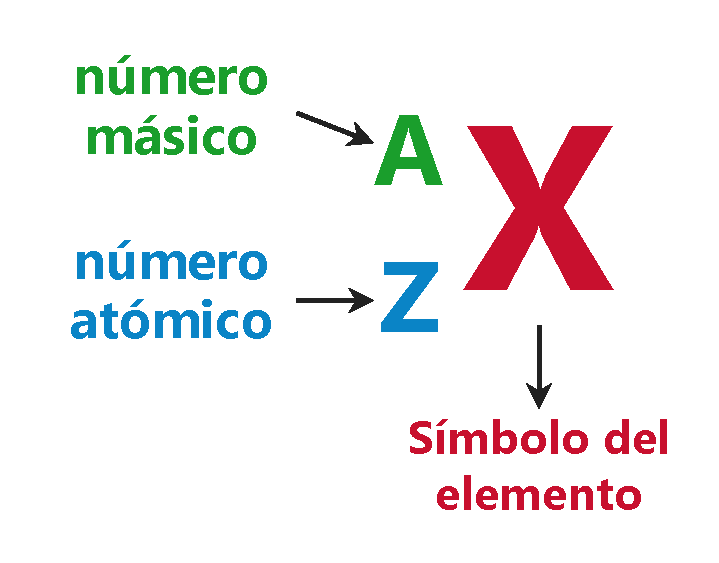
\includegraphics[width=0.8\linewidth]{Figuras_SVG_ES/pdf/U6_numero_masico_atomico.pdf}
        \caption{Representación del número másico y el número atómico}
        \label{fig:massatomic}
    \end{figure}
\end{minipage}
%\begin{figure}[H]
%    \centering
%    \includegraphics[scale=0.6]{images/SP_atomo/z_a_atomica_figura.pdf}
%    \caption{Representation of mass number and atomic number}
%    \label{fig:massatomic}
%\end{figure}
\begin{example}
    Vamos a determinar el número de protones, neutrones y electrones en los siguientes átomos neutros:
    \begin{itemize}
        \item \textbf{\isotope{Na} (Sodio):}
        \begin{itemize}
            \item Protones: \( Z = 11 \) → 11 protones
            \item Electrones: Al ser neutro, 11 electrones
            \item Neutrones: \( \ntr = A - Z = 23 - 11 = 12 \) neutrones
        \end{itemize}

        \item \textbf{\isotope{Po} (Polonio):}
        \begin{itemize}
            \item Protones: \( Z = 84 \) → 84 protones
            \item Electrones: Al ser neutro, 84 electrones
            \item Neutrones: \( \ntr = A - Z = 209 - 84 = 125 \) neutrones
        \end{itemize}
    \end{itemize}
\end{example}


\begin{exercise}
    Indica el número de protones, neutrones y electrones de un átomo de cloro \isotope{Cl}.

    \begin{solu}
        Para resolver este ejercicio, necesitamos interpretar la notación isotópica del cloro.

        A partir de la notación \isotope{Cl} obtenemos:
        \begin{itemize}
            \item Número másico (A) = 35 (parte superior)
            \item Número atómico (Z) = 17 (parte inferior)
        \end{itemize}

        \textbf{Paso 1: Calcular el número de protones}

        El número atómico (Z) indica directamente el número de protones:
        \[
            \text{Número de protones} = Z = 17
        \]

        \textbf{Paso 2: Calcular el número de neutrones}

        El número de neutrones se calcula restando el número atómico del número másico:
        \[
            \text{Número de neutrones} = A - Z = 35 - 17 = 18
        \]

        \textbf{Paso 3: Calcular el número de electrones}

        Dado que el ejercicio indica que se trata de un átomo (no un ion), es eléctricamente neutro. Por tanto, el número de electrones es igual al número de protones:
        \[
            \text{Número de electrones} = Z = 17
        \]

        \textbf{Respuesta:} El átomo de cloro-35 tiene \textbf{17 protones, 18 neutrones y 17 electrones}.
    \end{solu}
\end{exercise}
\begin{exercise}
    ¿Cómo representarías un átomo de potasio eléctricamente neutro si Z = 19 y A = 39? ¿Cuántos protones, neutrones y electrones tiene?
    \begin{solu}
        \textbf{Paso 1: Representación del átomo}

        Para representar un átomo utilizamos la notación \ch{^{A}_{Z}X}, donde:
        \begin{itemize}
            \item X = símbolo del elemento (K para potasio)
            \item A = número másico = 39
            \item Z = número atómico = 19
        \end{itemize}

        Por tanto, la representación es: \ch{^{39}_{19}K}

        \textbf{Paso 2: Calcular el número de protones}

        El número de protones es igual al número atómico:
        \[
            \text{Número de protones} = Z = 19
        \]

        \textbf{Paso 3: Calcular el número de neutrones}

        El número de neutrones se obtiene restando:
        \[
            \text{Número de neutrones} = A - Z = 39 - 19 = 20
        \]

        \textbf{Paso 4: Calcular el número de electrones}

        Dado que el átomo es eléctricamente neutro (no tiene carga), el número de electrones es igual al número de protones:
        \[
            \text{Número de electrones} = 19
        \]

        \textbf{Respuesta:} El átomo se representa como \ch{^{39}_{19}K} y tiene \textbf{19 protones, 20 neutrones y 19 electrones}.
    \end{solu}
\end{exercise}

\begin{exercise}
    ¿Podemos afirmar que Z siempre indica el número de electrones? Explica tu respuesta.
    \begin{solu}
        \textbf{Análisis del concepto:}

        El número atómico (Z) es una propiedad que define el elemento químico y representa el número de protones en el núcleo del átomo. Este valor es constante para cada elemento.

        \textbf{Caso 1: Átomo neutro}

        En un átomo eléctricamente neutro, la carga positiva de los protones debe estar exactamente compensada por la carga negativa de los electrones. Por tanto:
        \[
            \text{Número de electrones} = \text{Número de protones} = Z
        \]

        En este caso, \textbf{sí} podemos decir que Z indica el número de electrones.

        \textbf{Caso 2: Iones (átomos cargados)}

        Cuando un átomo gana o pierde electrones, se convierte en un ion:
        \begin{itemize}
            \item \textbf{Catión} (carga positiva): ha perdido electrones
            \[
                \text{Número de electrones} = Z - \text{carga positiva}
            \]
            Ejemplo: \ch{Na^{+}} tiene Z = 11, pero solo 10 electrones.

            \item \textbf{Anión} (carga negativa): ha ganado electrones
            \[
                \text{Número de electrones} = Z + \text{carga negativa}
            \]
            Ejemplo: \ch{Cl^{-}} tiene Z = 17, pero 18 electrones.
        \end{itemize}

        En estos casos, Z \textbf{no} indica el número de electrones.

        \textbf{Respuesta:} No siempre. Z indica el número de protones, que es igual al número de electrones SOLO si el átomo es neutro. Si el átomo tiene carga (es un ion), el número de electrones será diferente del valor de Z.
    \end{solu}
\end{exercise}
\begin{exercise}
    El número de neutrones del litio es una unidad más que el número de protones. Sabiendo que su número másico es 7:
    \begin{enumerate}[label=\letraminuscula]
    \item ¿Cuál es su número atómico?
    \item ¿Cuántos electrones tiene un átomo de litio eléctricamente neutro?
    \end{enumerate}
    \begin{solu}
        \textbf{Datos:}
        \begin{itemize}
            \item Número másico: A = 7
            \item Relación: número de neutrones = número de protones + 1
        \end{itemize}

        \textbf{Apartado a) Calcular el número atómico}

        \textbf{Paso 1:} Expresar la relación entre neutrones y protones

        Si llamamos Z al número de protones:
        \[
            \text{Número de neutrones} = Z + 1
        \]

        \textbf{Paso 2:} Utilizar la relación del número másico

        Sabemos que el número másico es la suma de protones y neutrones:
        \[
            A = \text{protones} + \text{neutrones}
        \]
        \[
            7 = Z + (Z + 1)
        \]

        \textbf{Paso 3:} Resolver la ecuación
        \[
            7 = 2Z + 1
        \]
        \[
            6 = 2Z
        \]
        \[
            Z = 3
        \]

        \textbf{Respuesta a):} El número atómico del litio es \textbf{Z = 3}.

        \textbf{Apartado b) Calcular el número de electrones}

        Dado que el ejercicio indica que el átomo es eléctricamente neutro, el número de electrones debe ser igual al número de protones para que las cargas se compensen:
        \[
            \text{Número de electrones} = Z = 3
        \]

        \textbf{Respuesta b):} Un átomo de litio eléctricamente neutro tiene \textbf{3 electrones}.

        \textbf{Verificación:}
        \begin{itemize}
            \item Protones: 3
            \item Neutrones: 3 + 1 = 4
            \item Número másico: 3 + 4 = 7 \( \checkmark \)
        \end{itemize}
    \end{solu}
\end{exercise}
\begin{exercise}
    Representa mediante la notación \ch{^{A}_{Z}X} indicando el número de protones, neutrones y electrones de los siguientes átomos:
    \begin{multicols}{2}
        \begin{enumerate}[label=\letraminuscula]
    \item Boro con 5 protones y 6 neutrones
    \item Nitrógeno con 7 protones y 7 neutrones
    \item Carbono con 6 protones y 6 neutrones
    \item Oxígeno con 8 protones y 8 neutrones
    \item Flúor con 9 protones y 10 neutrones
    \item Helio con 2 protones y 2 neutrones
        \end{enumerate}
    \end{multicols}
    \begin{solu}
        Para cada átomo seguiremos estos pasos:
        \begin{enumerate}
            \item Identificar Z (número de protones)
            \item Calcular A (número másico = protones + neutrones)
            \item Determinar el símbolo del elemento
            \item Calcular los electrones (igual a los protones si el átomo es neutro)
        \end{enumerate}

        \textbf{a) Boro con 5 protones y 6 neutrones}
        \begin{itemize}
            \item Z = 5 (protones)
            \item A = 5 + 6 = 11
            \item Símbolo: B
            \item Electrones = 5 (átomo neutro)
        \end{itemize}
        Representación: \ch{^{11}_{5}B}

        \textbf{Respuesta:} \ch{^{11}_{5}B} tiene 5 protones, 6 neutrones y 5 electrones.

        \textbf{b) Nitrógeno con 7 protones y 7 neutrones}
        \begin{itemize}
            \item Z = 7 (protones)
            \item A = 7 + 7 = 14
            \item Símbolo: N
            \item Electrones = 7 (átomo neutro)
        \end{itemize}
        Representación: \ch{^{14}_{7}N}

        \textbf{Respuesta:} \ch{^{14}_{7}N} tiene 7 protones, 7 neutrones y 7 electrones.

        \textbf{c) Carbono con 6 protones y 6 neutrones}
        \begin{itemize}
            \item Z = 6 (protones)
            \item A = 6 + 6 = 12
            \item Símbolo: C
            \item Electrones = 6 (átomo neutro)
        \end{itemize}
        Representación: \ch{^{12}_{6}C}

        \textbf{Respuesta:} \ch{^{12}_{6}C} tiene 6 protones, 6 neutrones y 6 electrones.

        \textbf{d) Oxígeno con 8 protones y 8 neutrones}
        \begin{itemize}
            \item Z = 8 (protones)
            \item A = 8 + 8 = 16
            \item Símbolo: O
            \item Electrones = 8 (átomo neutro)
        \end{itemize}
        Representación: \ch{^{16}_{8}O}

        \textbf{Respuesta:} \ch{^{16}_{8}O} tiene 8 protones, 8 neutrones y 8 electrones.

        \textbf{e) Flúor con 9 protones y 10 neutrones}
        \begin{itemize}
            \item Z = 9 (protones)
            \item A = 9 + 10 = 19
            \item Símbolo: F
            \item Electrones = 9 (átomo neutro)
        \end{itemize}
        Representación: \ch{^{19}_{9}F}

        \textbf{Respuesta:} \ch{^{19}_{9}F} tiene 9 protones, 10 neutrones y 9 electrones.

        \textbf{f) Helio con 2 protones y 2 neutrones}
        \begin{itemize}
            \item Z = 2 (protones)
            \item A = 2 + 2 = 4
            \item Símbolo: He
            \item Electrones = 2 (átomo neutro)
        \end{itemize}
        Representación: \ch{^{4}_{2}He}

        \textbf{Respuesta:} \ch{^{4}_{2}He} tiene 2 protones, 2 neutrones y 2 electrones.
    \end{solu}
\end{exercise}
\begin{exercise}
    Indica el número de protones, neutrones y electrones de los siguientes átomos:
    \begin{multicols}{5}
        \begin{enumerate}[label=\letraminuscula]
        \item \isotope{He}
        \item \isotope{F}
        \item \isotope{Ne}
        \item \isotope{Mg}
        \item \isotope{Ar}
        \end{enumerate}
    \end{multicols}
    \begin{solu}
        Para resolver este ejercicio, interpretaremos la notación isotópica de cada átomo y aplicaremos las siguientes fórmulas:
        \begin{itemize}
            \item Número de protones = Z (número atómico, parte inferior)
            \item Número de neutrones = A - Z (número másico - número atómico)
            \item Número de electrones = Z (si el átomo es neutro)
        \end{itemize}

        \textbf{a) \isotope{He}}
        \begin{itemize}
            \item Z = 2 (número atómico)
            \item A = 4 (número másico)
            \item Protones = 2
            \item Neutrones = 4 - 2 = 2
            \item Electrones = 2 (átomo neutro)
        \end{itemize}
        \textbf{Respuesta:} 2 protones, 2 neutrones, 2 electrones.

        \textbf{b) \isotope{F}}
        \begin{itemize}
            \item Z = 9 (número atómico)
            \item A = 19 (número másico)
            \item Protones = 9
            \item Neutrones = 19 - 9 = 10
            \item Electrones = 9 (átomo neutro)
        \end{itemize}
        \textbf{Respuesta:} 9 protones, 10 neutrones, 9 electrones.

        \textbf{c) \isotope{Ne}}
        \begin{itemize}
            \item Z = 10 (número atómico)
            \item A = 20 (número másico)
            \item Protones = 10
            \item Neutrones = 20 - 10 = 10
            \item Electrones = 10 (átomo neutro)
        \end{itemize}
        \textbf{Respuesta:} 10 protones, 10 neutrones, 10 electrones.

        \textbf{d) \isotope{Mg}}
        \begin{itemize}
            \item Z = 12 (número atómico)
            \item A = 24 (número másico)
            \item Protones = 12
            \item Neutrones = 24 - 12 = 12
            \item Electrones = 12 (átomo neutro)
        \end{itemize}
        \textbf{Respuesta:} 12 protones, 12 neutrones, 12 electrones.

        \textbf{e) \isotope{Ar}}
        \begin{itemize}
            \item Z = 18 (número atómico)
            \item A = 40 (número másico)
            \item Protones = 18
            \item Neutrones = 40 - 18 = 22
            \item Electrones = 18 (átomo neutro)
        \end{itemize}
        \textbf{Respuesta:} 18 protones, 22 neutrones, 18 electrones.

        \textbf{f) \isotope{Ca}}
        \begin{itemize}
            \item Z = 20 (número atómico)
            \item A = 40 (número másico)
            \item Protones = 20
            \item Neutrones = 40 - 20 = 20
            \item Electrones = 20 (átomo neutro)
        \end{itemize}
        \textbf{Respuesta:} 20 protones, 20 neutrones, 20 electrones.
    \end{solu}
\end{exercise}
\section{Iones}
\begin{definition}[ion]
    Es un átomo (o grupo de átomos) que ha ganado o perdido electrones y por tanto tiene una carga eléctrica.
\end{definition}
Cuando un átomo gana o pierde electrones, deja de ser neutro y se convierte en un ion:
\begin{itemize}
    \item \negsubro{Catión} (\textbf{ion positivo}): Se forma cuando un átomo \textbf{pierde electrones}. Al tener menos electrones que protones, queda con carga positiva. Se representa con el signo \( + \).

    Ejemplo: \ch{Na^{+}} (el sodio ha perdido 1 electrón)

    \item \negsubro{Anión} (\textbf{ion negativo}): Se forma cuando un átomo \textbf{gana electrones}. Al tener más electrones que protones, queda con carga negativa. Se representa con el signo \( - \).

    Ejemplo: \ch{Cl^{-}} (el cloro ha ganado 1 electrón)
\end{itemize}
\begin{remark}
    \textbf{Regla importante:} El número de protones (Z) \textbf{nunca cambia} cuando se forma un ion, porque los protones están en el núcleo y no se pueden ganar o perder fácilmente. Solo cambia el número de electrones.
\end{remark}
\begin{example}
    Vamos a determinar el número de protones, neutrones y electrones en los siguientes iones:

    \begin{itemize}
        \item \textbf{\isotope{23,11,Na}$^{+}$ (Catión sodio):}
        \begin{itemize}
            \item Protones: \( Z = 11 \) → 11 protones (no cambia)
            \item Neutrones: \( A - Z = 23 - 11 = 12 \) neutrones
            \item Electrones: 10 electrones (ha perdido 1 electrón: 11 - 1 = 10)
        \end{itemize}

        \item \textbf{\isotope{35,17,Cl}$^{-}$ (Anión cloro):}
        \begin{itemize}
            \item Protones: \( Z = 17 \) → 17 protones (no cambia)
            \item Neutrones: \( A - Z = 35 - 17 = 18 \) neutrones
            \item Electrones: 18 electrones (ha ganado 1 electrón: 17 + 1 = 18)
        \end{itemize}
    \end{itemize}
\end{example}
\begin{exercise}
    Indica el número de protones, neutrones y electrones de los siguientes iones:
    \begin{multicols}{4}
        \begin{enumerate}[label=\letraminuscula]
        \item \isotope{Ca}$^{2+}$
        \item \isotope{O}$^{2-}$
        \item \isotope{Al}$^{3+}$
        \item \isotope{S}$^{2-}$
        \end{enumerate}
    \end{multicols}
    \begin{solu}
        Para resolver este ejercicio, debemos recordar que:
        \begin{itemize}
            \item El número de protones es siempre igual a Z (número atómico) y no cambia.
            \item El número de neutrones = A - Z
            \item Para los iones:
            \begin{itemize}
                \item Cationes (carga positiva): han perdido electrones → electrones = Z - carga
                \item Aniones (carga negativa): han ganado electrones → electrones = Z + carga
            \end{itemize}
        \end{itemize}

        \textbf{a) \isotope{Ca}$^{2+}$}

        \textbf{Paso 1:} Identificar los datos a partir de la notación isotópica
        \begin{itemize}
            \item Z = 20 (número atómico del calcio)
            \item A = 40 (número másico)
            \item Carga = 2+ (catión)
        \end{itemize}

        \textbf{Paso 2:} Calcular los protones
        \[
            \text{Protones} = Z = 20
        \]

        \textbf{Paso 3:} Calcular los neutrones
        \[
            \text{Neutrones} = A - Z = 40 - 20 = 20
        \]

        \textbf{Paso 4:} Calcular los electrones

        Al ser un catión con carga 2+, ha perdido 2 electrones:
        \[
            \text{Electrones} = Z - 2 = 20 - 2 = 18
        \]

        \textbf{Respuesta:} 20 protones, 20 neutrones, 18 electrones.

        \textbf{b) \isotope{O}$^{2-}$}

        \textbf{Paso 1:} Identificar los datos a partir de la notación isotópica
        \begin{itemize}
            \item Z = 8 (número atómico del oxígeno)
            \item A = 16 (número másico)
            \item Carga = 2- (anión)
        \end{itemize}

        \textbf{Paso 2:} Calcular los protones
        \[
            \text{Protones} = Z = 8
        \]

        \textbf{Paso 3:} Calcular los neutrones
        \[
            \text{Neutrones} = A - Z = 16 - 8 = 8
        \]

        \textbf{Paso 4:} Calcular los electrones

        Al ser un anión con carga 2-, ha ganado 2 electrones:
        \[
            \text{Electrones} = Z + 2 = 8 + 2 = 10
        \]

        \textbf{Respuesta:} 8 protones, 8 neutrones, 10 electrones.

        \textbf{c) \isotope{Al}$^{3+}$}

        \textbf{Paso 1:} Identificar los datos a partir de la notación isotópica
        \begin{itemize}
            \item Z = 13 (número atómico del aluminio)
            \item A = 27 (número másico)
            \item Carga = 3+ (catión)
        \end{itemize}

        \textbf{Paso 2:} Calcular los protones
        \[
            \text{Protones} = Z = 13
        \]

        \textbf{Paso 3:} Calcular los neutrones
        \[
            \text{Neutrones} = A - Z = 27 - 13 = 14
        \]

        \textbf{Paso 4:} Calcular los electrones

        Al ser un catión con carga 3+, ha perdido 3 electrones:
        \[
            \text{Electrones} = Z - 3 = 13 - 3 = 10
        \]

        \textbf{Respuesta:} 13 protones, 14 neutrones, 10 electrones.

        \textbf{d) \isotope{S}$^{2-}$}

        \textbf{Paso 1:} Identificar los datos a partir de la notación isotópica
        \begin{itemize}
            \item Z = 16 (número atómico del azufre)
            \item A = 32 (número másico)
            \item Carga = 2- (anión)
        \end{itemize}

        \textbf{Paso 2:} Calcular los protones
        \[
            \text{Protones} = Z = 16
        \]

        \textbf{Paso 3:} Calcular los neutrones
        \[
            \text{Neutrones} = A - Z = 32 - 16 = 16
        \]

        \textbf{Paso 4:} Calcular los electrones

        Al ser un anión con carga 2-, ha ganado 2 electrones:
        \[
            \text{Electrones} = Z + 2 = 16 + 2 = 18
        \]

        \textbf{Respuesta:} 16 protones, 16 neutrones, 18 electrones.
    \end{solu}
\end{exercise}
\begin{exercise}
    ¿Cuántos electrones ha perdido o ganado un átomo de aluminio (\( Z = 13 \)) para convertirse en \ch{Al^{3+}}?
    \begin{solu}
        \textbf{Datos:}
        \begin{itemize}
            \item Número atómico del aluminio: Z = 13
            \item Ion formado: \ch{Al^{3+}}
            \item Carga del ion: 3+
        \end{itemize}

        \textbf{Paso 1:} Determinar el número de electrones en el átomo neutro

        Un átomo de aluminio eléctricamente neutro tiene el mismo número de electrones que de protones:
        \[
            \text{Electrones en el átomo neutro} = Z = 13
        \]

        \textbf{Paso 2:} Determinar el número de electrones en el ion

        El ion \ch{Al^{3+}} tiene una carga positiva de 3+, lo que significa que:
        \[
            \text{Electrones en el ion} = Z - 3 = 13 - 3 = 10
        \]

        \textbf{Paso 3:} Calcular cuántos electrones se han perdido o ganado

        Comparamos el número de electrones antes y después:
        \[
            \text{Electrones perdidos} = 13 - 10 = 3
        \]

        \textbf{Análisis del resultado:}

        Dado que la carga es positiva (3+), esto indica una pérdida de electrones, no una ganancia. El átomo de aluminio ha cedido 3 electrones para formar el catión \ch{Al^{3+}}.

        \textbf{Verificación:}
        \begin{itemize}
            \item Átomo neutro: 13 protones (+) y 13 electrones (-) → carga neta = 0
            \item Ion \ch{Al^{3+}}: 13 protones (+) y 10 electrones (-) → carga neta = +3 \( \checkmark \)
        \end{itemize}

        \textbf{Respuesta:} El átomo de aluminio ha \textbf{perdido 3 electrones} para convertirse en \ch{Al^{3+}}.
    \end{solu}
\end{exercise}
\section{Isótopos}
\begin{definition}[isótopos]
    Son átomos del mismo elemento químico (tienen el mismo número atómico \( Z \)) pero diferente número de neutrones y por tanto diferente número másico (\( A \)).
\end{definition}
\textbf{Características de los isótopos:}
\begin{itemize}
    \item Tienen el \textbf{mismo número de protones} (mismo \( Z \))
    \item Tienen \textbf{diferente número de neutrones}
    \item Tienen \textbf{diferente número másico} (\( A \))
    \item Son del \textbf{mismo elemento químico}
    \item Tienen \textbf{propiedades químicas muy similares}
\end{itemize}
\begin{example}
    El carbono tiene varios isótopos. Los más comunes son:
    \begin{itemize}
        \item \textbf{Carbono-12:} \isotope{C}
        \begin{itemize}
            \item 6 protones, 6 neutrones, 6 electrones
            \item Es el isótopo más abundante (98,9\%)
        \end{itemize}

        \item \textbf{Carbono-13:} \isotope{13,C}
        \begin{itemize}
            \item 6 protones, 7 neutrones, 6 electrones
            \item Menos abundante (1,1\%)
        \end{itemize}
        \item \textbf{Carbono-14:} \isotope{14,C}
        \begin{itemize}
            \item 6 protones, 8 neutrones, 6 electrones
            \item Es radiactivo y se utiliza para datar fósiles
        \end{itemize}
    \end{itemize}
    Los tres son carbono porque tienen 6 protones, pero se diferencian en el número de neutrones.
\end{example}
%\begin{remark}
%    \textbf{Practical application:} Carbon-14 is used to determine the age of archaeological remains and fossils. This method is called ``carbon-14 dating'' and has made it possible to determine the age of mummies, ancient scrolls, and prehistoric remains.
%\end{remark}
\begin{exercise}
    ¿Cuáles de los siguientes átomos son isótopos entre sí?
    \begin{multicols}{4}
        \begin{enumerate}[label=\letraminuscula]
        \item \isotope{Ne}
        \item \isotope{21,Ne}
        \item \isotope{F}
        \item \isotope{Na}
        \end{enumerate}
    \end{multicols}
    \begin{solu}
        \textbf{Concepto de isótopos:}

        Los isótopos son átomos del mismo elemento (mismo número atómico Z) que tienen diferente número de neutrones y por tanto diferente número másico (A).

        \textbf{Condición para ser isótopos:}
        \[
            \text{Mismo Z (número atómico)} \quad \text{y} \quad \text{Diferente A (número másico)}
        \]

        \textbf{Paso 1:} Analizar cada átomo e identificar Z y A

        \textbf{a) \isotope{Ne}}
        \begin{itemize}
            \item Elemento: Neón (Ne)
            \item Z = 10 (número atómico)
            \item A = 20 (número másico)
        \end{itemize}

        \textbf{b) \isotope{Ne}}
        \begin{itemize}
            \item Elemento: Neón (Ne)
            \item Z = 10 (número atómico)
            \item A = 22 (número másico)
        \end{itemize}

        \textbf{c) \isotope{F}}
        \begin{itemize}
            \item Elemento: Flúor (F)
            \item Z = 9 (número atómico)
            \item A = 19 (número másico)
        \end{itemize}

        \textbf{d) \isotope{Na}}
        \begin{itemize}
            \item Elemento: Sodio (Na)
            \item Z = 11 (número atómico)
            \item A = 23 (número másico)
        \end{itemize}

        \textbf{Paso 2:} Comparar los átomos para identificar los isótopos

        Organizamos los datos en una tabla:

        \begin{center}
            % --- tabla antigua ---
            % \begin{tabular}{|c|c|c|c|}
                % \hline
                % \textbf{Átomo} & \textbf{Elemento} & \textbf{Z} & \textbf{A} \\
                % \hline
                % a)            & Ne               & 10         & 20         \\
                % \hline
                % b)            & Ne               & 10         & 22         \\
                % \hline
                % c)            & F                & 9          & 19         \\
                % \hline
                % d)            & Na               & 11         & 23         \\
                % \hline
            % \end{tabular}
            % --- tabla nueva ---
            \begin{tabular}{@{}cccc@{}}
                \toprule
                \textbf{Átomo} & \textbf{Elemento} & \textbf{Z} & \textbf{A} \\
                \midrule
                a) & Ne & 10 & 20 \\[3pt]
                b) & Ne & 10 & 22 \\[3pt]
                c) & F & 9 & 19 \\[3pt]
                d) & Na & 11 & 23 \\
                \bottomrule
            \end{tabular}
        \end{center}

        \textbf{Paso 3:} Identificar los isótopos

        Buscamos átomos con el mismo Z pero diferente A:
        \begin{itemize}
            \item Los átomos \textbf{a)} y \textbf{b)} son ambos neón (Z = 10)
            \item Tienen diferente número másico: A = 20 y A = 22
            \item Por tanto, \textbf{cumplen la condición para ser isótopos}
        \end{itemize}

        Los átomos c) y d) son elementos diferentes (F y Na), por lo que no pueden ser isótopos entre sí ni de los anteriores.

        \textbf{Verificación adicional:}

        Para \isotope{Ne}:
        \begin{itemize}
            \item Protones = 10
            \item Neutrones = 20 - 10 = 10
        \end{itemize}

        Para \isotope{Ne}:
        \begin{itemize}
            \item Protones = 10
            \item Neutrones = 22 - 10 = 12
        \end{itemize}

        Mismo número de protones pero diferente número de neutrones. \( \checkmark \)

        \textbf{Respuesta:} Los átomos \textbf{a) y b)} son isótopos entre sí. Se trata de dos isótopos del neón: neón-20 y neón-22.
    \end{solu}
\end{exercise}

\begin{exercise}
    El hidrógeno tiene tres isótopos conocidos:
    \begin{itemize}
        \item Hidrógeno común: 1 protón, 0 neutrones
        \item Deuterio: 1 protón, 1 neutrón
        \item Tritio: 1 protón, 2 neutrones
    \end{itemize}
    Represéntalos utilizando la notación \ch{^{A}_{Z}X}.
    \begin{solu}
        Para representar cada isótopo, necesitamos calcular:
        \begin{itemize}
            \item Z = número de protones (siempre el mismo para los tres isótopos)
            \item A = número másico = protones + neutrones
            \item X = símbolo del elemento (H para hidrógeno)
        \end{itemize}

        \textbf{Isótopo 1: Hidrógeno común (Protio)}

        \textbf{Paso 1:} Identificar los datos
        \begin{itemize}
            \item Número de protones = 1
            \item Número de neutrones = 0
        \end{itemize}

        \textbf{Paso 2:} Calcular Z y A
        \[
            Z = \text{número de protones} = 1
        \]
        \[
            A = \text{protones} + \text{neutrones} = 1 + 0 = 1
        \]

        \textbf{Paso 3:} Representar con la notación
        \[
            \boxed{\ch{^{1}_{1}H}}
        \]

        \textbf{Isótopo 2: Deuterio}

        \textbf{Paso 1:} Identificar los datos
        \begin{itemize}
            \item Número de protones = 1
            \item Número de neutrones = 1
        \end{itemize}

        \textbf{Paso 2:} Calcular Z y A
        \[
            Z = \text{número de protones} = 1
        \]
        \[
            A = \text{protones} + \text{neutrones} = 1 + 1 = 2
        \]

        \textbf{Paso 3:} Representar con la notación
        \[
            \boxed{\ch{^{2}_{1}H}} \quad \text{(también representado como \ch{^{2}_{1}D})}
        \]

        \textbf{Isótopo 3: Tritio}

        \textbf{Paso 1:} Identificar los datos
        \begin{itemize}
            \item Número de protones = 1
            \item Número de neutrones = 2
        \end{itemize}

        \textbf{Paso 2:} Calcular Z y A
        \[
            Z = \text{número de protones} = 1
        \]
        \[
            A = \text{protones} + \text{neutrones} = 1 + 2 = 3
        \]

        \textbf{Paso 3:} Representar con la notación
        \[
            \boxed{\ch{^{3}_{1}H}} \quad \text{(también representado como \ch{^{3}_{1}T})}
        \]

        \textbf{Verificación de que son isótopos:}

        Los tres átomos cumplen la condición para ser isótopos:
        \begin{itemize}
            \item Mismo número atómico: Z = 1 (todos son hidrógeno) \( \checkmark \)
            \item Diferente número másico: A = 1, 2 y 3 respectivamente \( \checkmark \)
            \item Diferente número de neutrones: 0, 1 y 2 respectivamente \( \checkmark \)
        \end{itemize}

        \textbf{Respuesta:}
        \begin{itemize}
            \item Hidrógeno común (Protio): \ch{^{1}_{1}H}
            \item Deuterio: \ch{^{2}_{1}H} o \ch{^{2}_{1}D}
            \item Tritio: \ch{^{3}_{1}H} o \ch{^{3}_{1}T}
        \end{itemize}

        \textbf{Nota:} El deuterio y el tritio son tan importantes que tienen sus propios símbolos (D y T), aunque lo más habitual es usar H para todos los isótopos del hidrógeno.
    \end{solu}
\end{exercise}

\section{Configuración Electrónica}
Ya sabemos que los electrones se distribuyen alrededor del núcleo en diferentes niveles de energía, pero no lo hacen al azar. Los electrones se organizan en diferentes zonas o ``pisos'' alrededor del núcleo.
\begin{definition}{Configuración electrónica}
    La \textbf{configuración electrónica} es como la ``dirección postal'' de los electrones. Nos indica exactamente dónde está cada electrón dentro del átomo, mediante una serie de números y letras.
\end{definition}
\newpage

\subsection{Niveles de energía: las capas del átomo}
\begin{minipage}{0.45\textwidth}
    Imagina el átomo como un edificio de apartamentos donde el núcleo está en el centro y los electrones viven en diferentes pisos alrededor de él:
    \begin{itemize}
        \item Los electrones más cercanos al núcleo (piso 1) están más fuertemente atraídos hacia él
        \item Los electrones más alejados (pisos superiores) están menos atraídos
        \item Cada piso se llama \textbf{nivel de energía} y se numera del 1 al 7
    \end{itemize}
    \begin{remark}
        \textbf{Analogía útil:} Los niveles de energía son como las capas de una cebolla. La primera capa (la más interna) es el nivel 1, la segunda capa es el nivel 2, y así sucesivamente hasta un máximo de 7 capas.
    \end{remark}
\end{minipage}
\hfill
\begin{minipage}{0.45\textwidth}
    \begin{figure}[H]
        \centering
        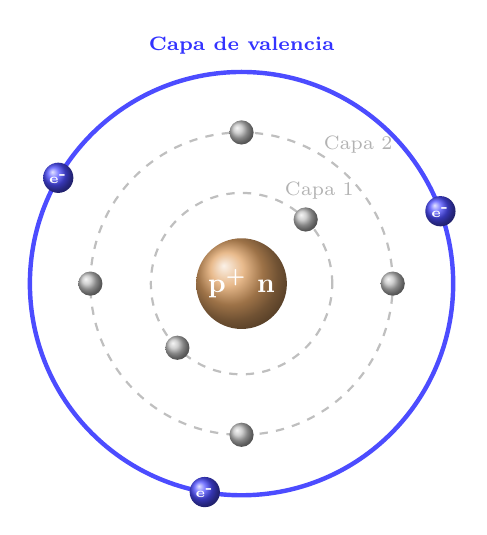
\begin{tikzpicture}[scale=0.48]
            % Núcleo con degradado ocre (solo p+ y n)
            \shade[ball color=orange!80!black!60] (0,0) circle (1.2cm);
            \node[font=\normalsize\bfseries, white] at (0,0) {p\textsuperscript{+} n};
            % Capa 1 (radio 2.4)
            \draw[gray!50, thick, dashed] (0,0) circle (2.4cm);
            % Etiqueta Capa 1: entre capa 1 (2.4) y capa 2 (4.0), a radio ~3.2
            \node[gray!60, font=\scriptsize] at (50:3.2) {Capa 1};
            % Capa 2 (radio 4.0, más separada)
            \draw[gray!50, thick, dashed] (0,0) circle (4.0cm);
            % Etiqueta Capa 2: entre capa 2 (4.0) y valencia (5.6), a radio ~4.8
            \node[gray!60, font=\scriptsize] at (50:4.8) {Capa 2};
            % Capa de valencia (radio 5.6, resaltada)
            \draw[blue!70, ultra thick] (0,0) circle (5.6cm);
            \node[blue!80, font=\scriptsize\bfseries] at (0, 6.3) {Capa de valencia};
            % Electrones de valencia (azules)
            \foreach \angle in {20, 150, 260} {
                \shade[ball color=blue!70] (\angle:5.6) circle (0.4cm);
                \node[white, font=\tiny\bfseries] at (\angle:5.6) {e\textsuperscript{-}};
            }
            % Electrones internos capa 1 (grises)
            \foreach \angle in {45, 225} {
                \shade[ball color=gray!50] (\angle:2.4) circle (0.32cm);
            }
            % Electrones internos capa 2 (grises)
            \foreach \angle in {0, 90, 180, 270} {
                \shade[ball color=gray!50] (\angle:4.0) circle (0.32cm);
            }
        \end{tikzpicture}
        \caption{Niveles de energía y capa de valencia.}
        \label{fig:niveles_capa_de_valencia}
    \end{figure}
\end{minipage}

\subsection{Orbitales: las habitaciones dentro de cada piso}
Dentro de cada nivel (cada piso), hay diferentes tipos de "habitaciones" donde pueden estar los electrones. Estas habitaciones se llaman \textbf{subniveles} u \textbf{orbitales} y se representan con letras: \textbf{s, p, d, f}
\begin{itemize}
    \item \textbf{Subnivel s}: El más sencillo, puede contener hasta \textbf{2 electrones} como máximo
    \item \textbf{Subnivel p}: Ligeramente más grande, puede contener hasta \textbf{6 electrones} como máximo
    \item \textbf{Subnivel d}: Más amplio, puede contener hasta \textbf{10 electrones} como máximo
    \item \textbf{Subnivel f}: El más grande, puede contener hasta \textbf{14 electrones} como máximo
\end{itemize}
\subsection{¿Qué orbitales hay en cada nivel?}
No todos los niveles tienen todos los tipos de orbitales. Aquí tienes la lista completa:
\begin{itemize}
    \item \textbf{Nivel 1}: solo tiene el orbital \textbf{s} → escribimos \( 1s \)
    \item \textbf{Nivel 2}: tiene los orbitales \textbf{s} y \textbf{p} → escribimos \( 2s, 2p \)
    \item \textbf{Nivel 3}: tiene \textbf{s, p} y \textbf{d} → escribimos \( 3s, 3p, 3d \)
    \item \textbf{Nivel 4}: tiene \textbf{s, p, d} y \textbf{f} → escribimos \( 4s, 4p, 4d, 4f \)
    \item \textbf{Niveles 5, 6 y 7}: igual que el nivel 4, tienen s, p, d y f
\end{itemize}
\begin{remark}
    \textbf{Patrón observable:} Cada nuevo nivel añade un tipo más de orbital. El nivel 1 solo tiene s, el nivel 2 añade p, el nivel 3 añade d, y el nivel 4 añade f.
\end{remark}
\subsection{Cómo se escriben los orbitales}
Cuando escribimos un orbital, utilizamos:
\begin{enumerate}
    \item Un \textbf{número} que indica el nivel (1, 2, 3, 4...)
    \item Una \textbf{letra} que indica el tipo de orbital (s, p, d, f)
    \item Un \textbf{exponente} (número pequeño arriba) que indica cuántos electrones hay en ese orbital
\end{enumerate}
\textbf{Ejemplos:}
\begin{itemize}
    \item \( 1s^2 \) → En el nivel 1, orbital s, hay 2 electrones
    \item \( 2p^6 \) → En el nivel 2, orbital p, hay 6 electrones
    \item \( 3d^{10} \) → En el nivel 3, orbital d, hay 10 electrones
    \item \( 3s^1 \) → En el nivel 3, orbital s, hay 1 electrón
\end{itemize}
\subsection{El Diagrama de Moeller: la guía para rellenar los orbitales}
Los electrones no rellenan los orbitales en el orden que podríamos pensar (primero 1s, luego 2s, luego 2p...). Existe un orden especial que debemos seguir, y para ello usamos el \textbf{Diagrama de Moeller}.
\begin{figure}[H]
    \centering
    \begin{tikzpicture}[>=stealth, font=\sffamily\LARGE\bfseries]

        % --- Configuración de Colores ---
        \definecolor{mygreen}{RGB}{0, 128, 0}
        \definecolor{myblue}{RGB}{91, 155, 213}

        % --- Dibujado de los Subniveles ---
        % Separación horizontal (2.2) y vertical (1.2) para que las diagonales sean perfectas
        \newcommand{\subnivel}[5]{
            \node (n#3#4) at (#1*2.2, -#2*1.2) {#3\textcolor{mygreen}{\textit{#4}}\textsuperscript{\textcolor{red}{#5}}};
        }

        % Columna s (x=0)
        \foreach \n in {1,...,7} \subnivel{0}{\n}{\n}{s}{2};
        % Columna p (x=1)
        \foreach \n in {2,...,7} \subnivel{1}{\n}{\n}{p}{6};
        % Columna d (x=2)
        \foreach \n in {3,...,7} \subnivel{2}{\n}{\n}{d}{10};
        % Columna f (x=3)
        \foreach \n in {4,...,7} \subnivel{3}{\n}{\n}{f}{14};

        % --- Dibujado de las Flechas Diagonales ---
        % Estilo: pasan por el centro, color azul, y se extienden 0.8cm hacia atrás y 1cm hacia adelante
        \tikzset{flecha/.style={myblue, very thick, *->, shorten <=-0.8cm, shorten >=-1cm}}

        % Para flechas que cruzan varios nodos (del centro del primero al centro del último)
        \draw[flecha] ($(n2p.center)+(1.5,0.7)$) -- (n3s.center);
        \draw[flecha] ($(n3p.center)+(1.5,0.7)$) -- (n4s.center);
        \draw[flecha] ($(n3d.center)+(1.5,0.7)$) -- (n5s.center);
        \draw[flecha] ($(n4d.center)+(1.5,0.7)$) -- (n6s.center);
        \draw[flecha] ($(n4f.center)+(1.5,0.7)$) -- (n7s.center);
        \draw[flecha] ($(n5f.center)+(1.5,0.7)$) -- (n7p.center);
        \draw[flecha] ($(n6f.center)+(1.5,0.7)$) -- (n7d.center);

        % Para las flechas de un solo nodo (1s, 2s y 7f), definimos una dirección manual
        % para que mantengan el mismo ángulo que las demás.
        \draw[flecha] ($(n1s.center)+(1.5,0.7)$) -- (n1s.center);
        \draw[flecha] ($(n2s.center)+(1.5,0.7)$) -- (n2s.center);
        \draw[flecha] (n7f.center) ++(1.5,0.8) -- (n7f.center);

    \end{tikzpicture}
    \caption{Diagrama de Moeller}
    \label{fig:diagrama_moeller}
\end{figure}
\begin{remark}
    \textbf{Cómo usar el Diagrama de Moeller:} Cada flecha te indica qué orbitales debes recorrer. Empiezas por la primera flecha (arriba a la izquierda) y sigues el recorrido de cada flecha. El orden que se obtiene es:
    \[
        1s \rightarrow 2s \rightarrow 2p \rightarrow 3s \rightarrow 3p \rightarrow 4s \rightarrow 3d \rightarrow 4p \rightarrow ...
    \]
\end{remark}
\subsection{Cómo escribir una configuración electrónica paso a paso}
Vamos a aprender a escribir la configuración electrónica del \textbf{Sodio (Na)} que tiene \( Z = 11 \), es decir, 11 electrones.
\begin{enumerate}[label=\textbf{Paso \arabic*:}]
        \item \textbf{Identificar cuántos electrones tiene el átomo}

        El sodio tiene \( Z = 11 \), por tanto tiene \textbf{11 electrones} que debemos colocar.

        \item \textbf{Seguir el diagrama de Moeller y rellenar los orbitales en orden}

        \begin{itemize}
            \item Las flechas siempre se siguen desde el punto de partida hasta la punta de flecha, comprobando los orbitales por los que pasamos hasta llegar a la punta.

            \item Primera flecha: En este caso solo pasa por \( 1s \): Este orbital puede tener un máximo de 2 electrones. Escribimos \( 1s^2 \)

            Electrones colocados: 2. Nos quedan: 11 - 2 = 9 electrones.

            \item Segunda flecha: Tenemos la misma situación y solo pasa por \( 2s \). Este orbital puede tener un máximo de 2 electrones. Escribimos \( 2s^2 \)

            Electrones colocados: 2 (de \( 1s \)) + 2 (de \( 2s \)) = 4. Nos quedan: 11 - 4 = 7 electrones.

            \item Tercera flecha: ahora pasa por \( 2p \) y \( 3s \): Primero colocamos los electrones en el orbital \( 2p \) porque es el primero en rellenarse y como podemos colocar un máximo de \num{6} electrones entonces escribimos: \( 2p^6 \). Ahora solo nos queda 1 electrón por colocar. El siguiente orbital según la flecha será \( 3s \), en este caso podríamos poner un máximo de \num{2} electrones pero como solo nos queda \num{1} electrón por colocar entonces debemos escribir: \( 3s^1 \)

            Electrones colocados: 2 (de \( 1s \)) + 2 (de \( 2s \)) + 6 (de \( 2p \)) + 1 (de \( 3s \)) = 11. ¡Perfecto! Los hemos colocado todos

            Electrones colocados: 10 + 1 = 11.
        \end{itemize}

        \item \textbf{Escribir la configuración electrónica completa}
        \[
            \text{Configuración del Na: } 1s^2\ 2s^2\ 2p^6\ 3s^1
        \]
\end{enumerate}
\begin{remark}
    \textbf{Consejo importante:} Cuenta siempre los electrones después de cada paso para asegurarte de que no superas el número total de electrones del átomo.
\end{remark}
\begin{example}
    \textbf{Configuración electrónica del Rubidio (Rb)} con \( Z = 37 \):
    Siguiendo el diagrama de Moeller y contando 37 electrones:
    \[
        1s^2\ 2s^2\ 2p^6\ 3s^2\ 3p^6\ 4s^2\ 3d^{10}\ 4p^6\ 5s^1
    \]

    Observa que el orbital \( 3d \) se rellena \textbf{después} de \( 4s \), aunque 3 sea menor que 4. Esto es lo que indica el diagrama de Moeller.
    \textbf{Reordenado por niveles} (opcional, pero más organizado):
    \[
        1s^2\ 2s^2\ 2p^6\ 3s^2\ 3p^6\ 3d^{10}\ 4s^2\ 4p^6\ 5s^1
    \]
\end{example}
\subsection{Configuración electrónica de los iones}
Cuando un átomo se convierte en ion (gana o pierde electrones), su configuración electrónica cambia:
\begin{itemize}
    \item \textbf{Para los cationes} (iones positivos, han perdido electrones):

    Primero se escribe la configuración del átomo neutro, y después \textbf{se quitan electrones desde el final} (desde el orbital con el número más alto).

    \textbf{Ejemplo:} \ch{Na^{+}} (ha perdido 1 electrón)
    \begin{itemize}
        \item Na neutro: \( 1s^2\ 2s^2\ 2p^6\ 3s^1 \)
        \item \ch{Na^{+}}: \( 1s^2\ 2s^2\ 2p^6 \) (quitamos 1 electrón de \( 3s \))
    \end{itemize}

    \item \textbf{Para los aniones} (iones negativos, han ganado electrones):
    Primero se escribe la configuración del átomo neutro, y después \textbf{se añaden electrones} siguiendo el orden del diagrama de Moeller.

    \textbf{Ejemplo:} \ch{Cl^{-}} (ha ganado 1 electrón)
    \begin{itemize}
        \item Cl neutro (\( Z = 17 \)): \( 1s^2\ 2s^2\ 2p^6\ 3s^2\ 3p^5 \)
        \item \ch{Cl^{-}}: \( 1s^2\ 2s^2\ 2p^6\ 3s^2\ 3p^6 \) (añadimos 1 electrón a \( 3p \))
    \end{itemize}
\end{itemize}
\begin{exercise}
    Escribe la configuración electrónica del Carbono (\( Z = 6 \)) en su estado fundamental (no pierde ni gana \el{}).

    \begin{solu}
        \textbf{Datos:}
        \begin{itemize}
            \item Elemento: Carbono (C)
            \item Número atómico: Z = 6
            \item Estado: Átomo neutro (no pierde ni gana electrones)
        \end{itemize}

        \textbf{Paso 1:} Determinar el número de electrones

        Dado que el átomo está en estado fundamental y es neutro:
        \[
            \text{Número de electrones} = Z = 6
        \]

        \textbf{Paso 2:} Recordar el orden de llenado de los orbitales

        Según el principio de Aufbau, los orbitales se rellenan en orden de energía creciente:
        \[
            1s \rightarrow 2s \rightarrow 2p \rightarrow 3s \rightarrow 3p \rightarrow 4s \rightarrow 3d \rightarrow \ldots
        \]

        \textbf{Paso 3:} Aplicar las reglas de llenado

        \textbf{Regla 1 - Principio de Aufbau:} Rellenar desde el orbital de menor energía.

        \textbf{Regla 2 - Principio de exclusión de Pauli:} Cada orbital puede contener un máximo de 2 electrones con espines opuestos.

        \textbf{Regla 3 - Regla de Hund:} En orbitales de igual energía, se coloca un electrón en cada orbital antes de emparejarlos.

        \textbf{Paso 4:} Distribuir los 6 electrones

        \begin{itemize}
            \item \textbf{Orbital 1s:} Contiene 2 electrones → \(1s^2\) (quedan 4 electrones)
            \item \textbf{Orbital 2s:} Contiene 2 electrones → \(2s^2\) (quedan 2 electrones)
            \item \textbf{Orbitales 2p:} Los 2 electrones restantes van a los orbitales 2p

            El subnivel 2p tiene 3 orbitales (2p\(_x\), 2p\(_y\), 2p\(_z\)), cada uno puede contener 2 electrones (total 6).

            Según la regla de Hund, primero se coloca un electrón en cada orbital:
            \[
                2p^2 \quad (\uparrow \quad \uparrow \quad \cdot)
            \]
        \end{itemize}

        \textbf{Paso 5:} Escribir la configuración electrónica completa
        \[
            \boxed{1s^2 \, 2s^2 \, 2p^2}
        \]

        \textbf{Verificación:}
        \[
            2 + 2 + 2 = 6 \text{ electrones} \quad \checkmark
        \]

        \textbf{Respuesta:} La configuración electrónica del carbono es: \elconf{C}
    \end{solu}
\end{exercise}
\begin{exercise}
    Determina la configuración electrónica del Fósforo (\( Z = 15 \)).
    \begin{solu}
        \textbf{Datos:}
        \begin{itemize}
            \item Elemento: Fósforo (P)
            \item Número atómico: Z = 15
            \item Estado: Átomo neutro
        \end{itemize}

        \textbf{Paso 1:} Determinar el número de electrones
        \[
            \text{Número de electrones} = Z = 15
        \]

        \textbf{Paso 2:} Orden de llenado de los orbitales

        Para 15 electrones necesitamos:
        \[
            1s \rightarrow 2s \rightarrow 2p \rightarrow 3s \rightarrow 3p
        \]

        \textbf{Paso 3:} Distribuir los 15 electrones siguiendo las reglas

        \begin{itemize}
            \item \textbf{Capa n = 1:}
            \begin{itemize}
                \item \(1s^2\) → 2 electrones (quedan 13)
            \end{itemize}

            \item \textbf{Capa n = 2:}
            \begin{itemize}
                \item \(2s^2\) → 2 electrones (quedan 11)
                \item \(2p^6\) → 6 electrones (quedan 5)
            \end{itemize}

            \item \textbf{Capa n = 3:}
            \begin{itemize}
                \item \(3s^2\) → 2 electrones (quedan 3)
                \item \(3p^3\) → 3 electrones (quedan 0)

                Los 3 electrones en 3p se distribuyen según Hund:
                \[
                    3p^3 \quad (\uparrow \quad \uparrow \quad \uparrow)
                \]
                Un electrón en cada orbital antes de emparejarlos.
            \end{itemize}
        \end{itemize}

        \textbf{Paso 4:} Escribir la configuración electrónica completa
        \[
            \boxed{1s^2 \, 2s^2 \, 2p^6 \, 3s^2 \, 3p^3}
        \]

        \textbf{Verificación:}
        \[
            2 + 2 + 6 + 2 + 3 = 15 \text{ electrones} \quad \checkmark
        \]

        \textbf{Forma simplificada (configuración del núcleo interno):}

        Podemos usar el gas noble anterior (Neón, Z = 10):
        \[
            \text{P:} \quad [\text{Ne}] \, 3s^2 \, 3p^3
        \]

        \textbf{Respuesta:} La configuración electrónica del fósforo es: \elconf{P}
    \end{solu}
\end{exercise}
\begin{exercise}
    Indica la configuración electrónica del anión cloruro \ch{Cl^{-}} (\( Z = 17 \)).
    \begin{solu}
        \textbf{Datos:}
        \begin{itemize}
            \item Elemento: Cloro (Cl)
            \item Número atómico: Z = 17
            \item Ion: \ch{Cl^{-}} (anión con carga 1-)
        \end{itemize}

        \textbf{Paso 1:} Determinar el número de electrones en el ion

        El átomo de cloro neutro tiene 17 electrones. Al ser un anión con carga 1-, ha ganado 1 electrón:
        \[
            \text{Número de electrones} = Z + 1 = 17 + 1 = 18
        \]

        \textbf{Paso 2:} Configuración del átomo de cloro neutro (17 e\(^-\))

        Primero escribimos la configuración del átomo neutro:
        \[
            \text{Cl:} \quad 1s^2 \, 2s^2 \, 2p^6 \, 3s^2 \, 3p^5
        \]

        \textbf{Paso 3:} Añadir el electrón adicional

        El electrón adicional se coloca en el siguiente orbital disponible según el orden de energía. Como 3p puede contener hasta 6 electrones y solo tiene 5, el electrón adicional completa este subnivel:
        \[
            3p^5 + 1e^- \rightarrow 3p^6
        \]

        \textbf{Paso 4:} Escribir la configuración electrónica del ion
        \[
            \boxed{\ch{Cl^{-}:} \quad 1s^2 \, 2s^2 \, 2p^6 \, 3s^2 \, 3p^6}
        \]

        \textbf{Verificación:}
        \[
            2 + 2 + 6 + 2 + 6 = 18 \text{ electrones} \quad \checkmark
        \]

        \textbf{Observación importante:}

        El ion \ch{Cl^{-}} tiene la misma configuración electrónica que el Argón (Ar, Z = 18), un gas noble. Decimos que el ion cloruro es isoelectrónico con el argón:
        \[
            \ch{Cl^{-}:} \quad [\text{Ar}] \quad \text{o} \quad 1s^2 \, 2s^2 \, 2p^6 \, 3s^2 \, 3p^6
        \]

        \textbf{Respuesta:} La configuración electrónica del anión cloruro es: \writeelconf{2,2+6,2+6}
    \end{solu}
\end{exercise}
\begin{exercise}
    Escribe la configuración electrónica del ion óxido \ch{O^{2-}} (\( Z = 8 \)).
    \begin{solu}
        \textbf{Datos:}
        \begin{itemize}
            \item Elemento: Oxígeno (O)
            \item Número atómico: Z = 8
            \item Ion: \ch{O^{2-}} (anión con carga 2-)
        \end{itemize}

        \textbf{Paso 1:} Determinar el número de electrones en el ion

        El átomo de oxígeno neutro tiene 8 electrones. Al ser un anión con carga 2-, ha ganado 2 electrones:
        \[
            \text{Número de electrones} = Z + 2 = 8 + 2 = 10
        \]

        \textbf{Paso 2:} Configuración del átomo de oxígeno neutro (8 e\(^-\))

        Primero escribimos la configuración del átomo neutro:
        \[
            \text{O:} \quad 1s^2 \, 2s^2 \, 2p^4
        \]

        Distribución de electrones:
        \begin{itemize}
            \item Capa 1: \(1s^2\) → 2 electrones
            \item Capa 2: \(2s^2\) → 2 electrones
            \item Capa 2: \(2p^4\) → 4 electrones
        \end{itemize}

        \textbf{Paso 3:} Añadir los 2 electrones adicionales

        Los 2 electrones adicionales se colocan en el subnivel 2p, que puede contener hasta 6 electrones:
        \[
            2p^4 + 2e^- \rightarrow 2p^6
        \]

        \textbf{Paso 4:} Escribir la configuración electrónica del ion
        \[
            \boxed{\ch{O^{2-}:} \quad 1s^2 \, 2s^2 \, 2p^6}
        \]

        \textbf{Verificación:}
        \[
            2 + 2 + 6 = 10 \text{ electrones} \quad \checkmark
        \]

        \textbf{Observación importante:}

        El ion óxido \ch{O^{2-}} tiene la misma configuración electrónica que el Neón (Ne, Z = 10), un gas noble. Es isoelectrónico con el neón y tiene una configuración muy estable:
        \[
            \ch{O^{2-}:} \quad [\text{Ne}] \quad \text{o} \quad 1s^2 \, 2s^2 \, 2p^6
        \]

        Esta configuración es especialmente estable porque completa la segunda capa electrónica.

        \textbf{Respuesta:} La configuración electrónica del ion óxido es: \writeelconf{2,2+6}
    \end{solu}
\end{exercise}
\begin{exercise}
    Determina la configuración electrónica del anión sulfuro \ch{S^{2-}} (\( Z = 16 \)).
    \begin{solu}
        \textbf{Datos:}
        \begin{itemize}
            \item Elemento: Azufre (S)
            \item Número atómico: Z = 16
            \item Ion: \ch{S^{2-}} (anión con carga 2-)
        \end{itemize}

        \textbf{Paso 1:} Determinar el número de electrones en el ion

        El átomo de azufre neutro tiene 16 electrones. Al ser un anión con carga 2-, ha ganado 2 electrones:
        \[
            \text{Número de electrones} = Z + 2 = 16 + 2 = 18
        \]

        \textbf{Paso 2:} Configuración del átomo de azufre neutro (16 e\(^-\))

        Primero escribimos la configuración del átomo neutro:
        \[
            \text{S:} \quad 1s^2 \, 2s^2 \, 2p^6 \, 3s^2 \, 3p^4
        \]

        Distribución de electrones:
        \begin{itemize}
            \item Capa 1: \(1s^2\) → 2 electrones
            \item Capa 2: \(2s^2 \, 2p^6\) → 8 electrones
            \item Capa 3: \(3s^2 \, 3p^4\) → 6 electrones
        \end{itemize}

        \textbf{Paso 3:} Añadir los 2 electrones adicionales

        Los 2 electrones adicionales se colocan en el subnivel 3p, que puede contener hasta 6 electrones y actualmente tiene 4:
        \[
            3p^4 + 2e^- \rightarrow 3p^6
        \]

        \textbf{Paso 4:} Escribir la configuración electrónica del ion
        \[
            \boxed{\ch{S^{2-}:} \quad 1s^2 \, 2s^2 \, 2p^6 \, 3s^2 \, 3p^6}
        \]

        \textbf{Verificación:}
        \[
            2 + 2 + 6 + 2 + 6 = 18 \text{ electrones} \quad \checkmark
        \]

        \textbf{Observación importante:}

        El ion sulfuro \ch{S^{2-}} tiene la misma configuración electrónica que el Argón (Ar, Z = 18), un gas noble. Es isoelectrónico con el argón:
        \[
            \ch{S^{2-}:} \quad [\text{Ar}] \quad \text{o} \quad 1s^2 \, 2s^2 \, 2p^6 \, 3s^2 \, 3p^6
        \]

        Esta configuración es muy estable porque completa la tercera capa con 8 electrones (regla del octeto).

        \textbf{Respuesta:} La configuración electrónica del anión sulfuro es: \writeelconf{2,2+6,2+6}
    \end{solu}
\end{exercise}
\begin{exercise}
    Escribe la configuración electrónica del catión sodio \ch{Na^{+}} (\( Z = 11 \)).
    \begin{solu}
        \textbf{Datos:}
        \begin{itemize}
            \item Elemento: Sodio (Na)
            \item Número atómico: Z = 11
            \item Ion: \ch{Na^{+}} (catión con carga 1+)
        \end{itemize}

        \textbf{Paso 1:} Determinar el número de electrones en el ion

        El átomo de sodio neutro tiene 11 electrones. Al ser un catión con carga 1+, ha perdido 1 electrón:
        \[
            \text{Número de electrones} = Z - 1 = 11 - 1 = 10
        \]

        \textbf{Paso 2:} Configuración del átomo de sodio neutro (11 e\(^-\))

        Primero escribimos la configuración del átomo neutro:
        \[
            \text{Na:} \quad 1s^2 \, 2s^2 \, 2p^6 \, 3s^1
        \]

        Distribución de electrones:
        \begin{itemize}
            \item Capa 1: \(1s^2\) → 2 electrones
            \item Capa 2: \(2s^2 \, 2p^6\) → 8 electrones
            \item Capa 3: \(3s^1\) → 1 electrón
        \end{itemize}

        \textbf{Paso 3:} Quitar el electrón perdido

        Cuando un átomo pierde electrones, los pierde de la capa más externa (el nivel de energía más alto). El sodio pierde su único electrón de la capa 3:
        \[
            3s^1 - 1e^- \rightarrow 3s^0 \quad \text{(eliminado)}
        \]

        \textbf{Paso 4:} Escribir la configuración electrónica del ion
        \[
            \boxed{\ch{Na^{+}:} \quad 1s^2 \, 2s^2 \, 2p^6}
        \]

        \textbf{Verificación:}
        \[
            2 + 2 + 6 = 10 \text{ electrones} \quad \checkmark
        \]

        \textbf{Observación importante:}

        El catión \ch{Na^{+}} tiene la misma configuración electrónica que el Neón (Ne, Z = 10), un gas noble. Es isoelectrónico con el neón:
        \[
            \ch{Na^{+}:} \quad [\text{Ne}] \quad \text{o} \quad 1s^2 \, 2s^2 \, 2p^6
        \]

        Al perder su electrón de valencia (\(3s^1\)), el sodio alcanza la configuración estable de gas noble, por lo que tiende a formar el catión \ch{Na^{+}} fácilmente.

        \textbf{Respuesta:} La configuración electrónica del catión sodio es: \writeelconf{2,2+6}
    \end{solu}
\end{exercise}
\begin{exercise}
    Indica la configuración electrónica del ion calcio \ch{Ca^{2+}} (\( Z = 20 \)).
    \begin{solu}
        \textbf{Datos:}
        \begin{itemize}
            \item Elemento: Calcio (Ca)
            \item Número atómico: Z = 20
            \item Ion: \ch{Ca^{2+}} (catión con carga 2+)
        \end{itemize}

        \textbf{Paso 1:} Determinar el número de electrones en el ion

        El átomo de calcio neutro tiene 20 electrones. Al ser un catión con carga 2+, ha perdido 2 electrones:
        \[
            \text{Número de electrones} = Z - 2 = 20 - 2 = 18
        \]

        \textbf{Paso 2:} Configuración del átomo de calcio neutro (20 e\(^-\))

        Primero escribimos la configuración del átomo neutro:
        \[
            \text{Ca:} \quad 1s^2 \, 2s^2 \, 2p^6 \, 3s^2 \, 3p^6 \, 4s^2
        \]

        Distribución de electrones:
        \begin{itemize}
            \item Capa 1: \(1s^2\) → 2 electrones
            \item Capa 2: \(2s^2 \, 2p^6\) → 8 electrones
            \item Capa 3: \(3s^2 \, 3p^6\) → 8 electrones
            \item Capa 4: \(4s^2\) → 2 electrones
        \end{itemize}

        \textbf{Paso 3:} Quitar los 2 electrones perdidos

        Los electrones se pierden de la capa más externa (el nivel de energía más alto). El calcio pierde sus 2 electrones de la capa 4:
        \[
            4s^2 - 2e^- \rightarrow 4s^0 \quad \text{(eliminados)}
        \]

        \textbf{Paso 4:} Escribir la configuración electrónica del ion
        \[
            \boxed{\ch{Ca^{2+}:} \quad 1s^2 \, 2s^2 \, 2p^6 \, 3s^2 \, 3p^6}
        \]

        \textbf{Verificación:}
        \[
            2 + 2 + 6 + 2 + 6 = 18 \text{ electrones} \quad \checkmark
        \]

        \textbf{Observación importante:}

        El catión \ch{Ca^{2+}} tiene la misma configuración electrónica que el Argón (Ar, Z = 18), un gas noble. Es isoelectrónico con el argón:
        \[
            \ch{Ca^{2+}:} \quad [\text{Ar}] \quad \text{o} \quad 1s^2 \, 2s^2 \, 2p^6 \, 3s^2 \, 3p^6
        \]

        Al perder sus 2 electrones de valencia (\(4s^2\)), el calcio alcanza la configuración estable de gas noble con 8 electrones en su capa más externa (regla del octeto), por lo que tiende a formar el catión \ch{Ca^{2+}} fácilmente.

        \textbf{Respuesta:} La configuración electrónica del ion calcio es: \writeelconf{2,2+6,2+6}
    \end{solu}
\end{exercise}
\subsection{Capa de valencia y electrones de valencia}
La capa o nivel más externo de un átomo es muy importante porque determina cómo se comportará ese átomo químicamente.
\begin{definition}{Capa de valencia}
    La \textbf{capa de valencia} es el nivel de energía más alto (el número más grande) que tiene electrones. Es la capa más externa del átomo.
\end{definition}
\begin{definition}{Electrones de valencia}
    Los \textbf{electrones de valencia} son todos los electrones que se encuentran en la capa de valencia. Son los electrones más externos y son los que participan en las reacciones químicas.
\end{definition}
\begin{remark}
    \textbf{¿Por qué son importantes los electrones de valencia?} Son como las ``manos'' del átomo: con ellas puede formar enlaces químicos con otros átomos. Los electrones internos están demasiado cerca del núcleo y no participan en las reacciones.
\end{remark}
\begin{example}
    \textbf{Sodio (Na):} \( 1s^2\ 2s^2\ 2p^6\ 3s^1 \)
    \begin{itemize}
        \item Capa de valencia: \textbf{n = 3} (el número más alto que aparece)
        \item Electrones de valencia: \textbf{1 electrón} (el de \( 3s^1 \))
    \end{itemize}

    \textbf{Oxígeno (O):} \( 1s^2\ 2s^2\ 2p^4 \)
    \begin{itemize}
        \item Capa de valencia: \textbf{n = 2}
        \item Electrones de valencia: \textbf{6 electrones} (2 en \( 2s \) + 4 en \( 2p \) = 6)
    \end{itemize}

    \textbf{Carbono (C):} \( 1s^2\ 2s^2\ 2p^2 \)
    \begin{itemize}
        \item Capa de valencia: \textbf{n = 2}
        \item Electrones de valencia: \textbf{4 electrones} (2 en \( 2s \) + 2 en \( 2p \) = 4)
    \end{itemize}
\end{example}
\begin{remark}
    \textbf{Conexión con la tabla periódica:} Los elementos del mismo grupo (misma columna) tienen el mismo número de electrones de valencia. Por eso tienen propiedades químicas similares. ¡Lo veremos en la siguiente sección!
\end{remark}
\begin{exercise}
    Identifica la capa de valencia y el número de electrones de valencia del Litio (\( Z = 3 \)).
    \begin{solu}
        \textbf{Datos:}
        \begin{itemize}
            \item Elemento: Litio (Li)
            \item Número atómico: Z = 3
            \item Estado: Átomo neutro
        \end{itemize}

        \textbf{Paso 1:} Determinar el número de electrones
        \[
            \text{Número de electrones} = Z = 3
        \]

        \textbf{Paso 2:} Escribir la configuración electrónica

        Distribuimos los 3 electrones siguiendo el orden de llenado:
        \begin{itemize}
            \item Orbital \(1s\): 2 electrones → \(1s^2\)
            \item Orbital \(2s\): 1 electrón → \(2s^1\)
        \end{itemize}

        Configuración electrónica completa:
        \[
            \text{Li:} \quad 1s^2 \, 2s^1
        \]

        \textbf{Verificación:}
        \[
            2 + 1 = 3 \text{ electrones} \quad \checkmark
        \]

        \textbf{Paso 3:} Identificar la capa de valencia

        La capa de valencia es la capa más externa (con el número cuántico principal \(n\) más alto).

        Analizando la configuración:
        \begin{itemize}
            \item Capa 1 (\(n = 1\)): \(1s^2\) → capa completa (interna)
            \item Capa 2 (\(n = 2\)): \(2s^1\) → capa más externa
        \end{itemize}

        Por tanto, la capa de valencia es:
        \[
            \boxed{n = 2}
        \]

        \textbf{Paso 4:} Contar los electrones de valencia

        Los electrones de valencia son los que se encuentran en la capa más externa:
        \[
            \text{Electrones en la capa } n = 2: \quad 2s^1 \rightarrow 1 \text{ electrón}
        \]

        Por tanto:
        \[
            \boxed{\text{Electrones de valencia} = 1}
        \]

        \textbf{Respuesta:}
        \begin{itemize}
            \item Configuración electrónica: \elconf{Li}
            \item Capa de valencia: \(n = 2\)
            \item Electrones de valencia: 1
        \end{itemize}
    \end{solu}
\end{exercise}
\begin{exercise}
    Determina la capa de valencia y los electrones de valencia del Nitrógeno (\( Z = 7 \)).
    \begin{solu}
        \textbf{Datos:}
        \begin{itemize}
            \item Elemento: Nitrógeno (N)
            \item Número atómico: Z = 7
            \item Estado: Átomo neutro
        \end{itemize}

        \textbf{Paso 1:} Determinar el número de electrones
        \[
            \text{Número de electrones} = Z = 7
        \]

        \textbf{Paso 2:} Escribir la configuración electrónica

        Distribuimos los 7 electrones siguiendo el orden de llenado:
        \begin{itemize}
            \item Capa 1 (\(n = 1\)):
            \begin{itemize}
                \item \(1s^2\) → 2 electrones
            \end{itemize}
            \item Capa 2 (\(n = 2\)):
            \begin{itemize}
                \item \(2s^2\) → 2 electrones
                \item \(2p^3\) → 3 electrones
            \end{itemize}
        \end{itemize}

        Configuración electrónica completa:
        \[
            \text{N:} \quad 1s^2 \, 2s^2 \, 2p^3
        \]

        \textbf{Verificación:}
        \[
            2 + 2 + 3 = 7 \text{ electrones} \quad \checkmark
        \]

        \textbf{Paso 3:} Identificar la capa de valencia

        La capa de valencia es la capa más externa.

        Analizando la configuración:
        \begin{itemize}
            \item Capa 1 (\(n = 1\)): \(1s^2\) → capa completa (interna)
            \item Capa 2 (\(n = 2\)): \(2s^2 \, 2p^3\) → capa más externa
        \end{itemize}

        Por tanto, la capa de valencia es:
        \[
            \boxed{n = 2}
        \]

        \textbf{Paso 4:} Contar los electrones de valencia

        Los electrones de valencia son todos los electrones de la capa más externa:
        \[
            \text{Electrones en la capa } n = 2: \quad 2s^2 + 2p^3 = 2 + 3 = 5 \text{ electrones}
        \]

        Por tanto:
        \[
            \boxed{\text{Electrones de valencia} = 5}
        \]

        \textbf{Observación:}

        El nitrógeno tiene 5 electrones de valencia, lo que significa que necesita 3 electrones para completar su capa de valencia (regla del octeto). Por eso tiende a formar 3 enlaces covalentes.

        \textbf{Respuesta:}
        \begin{itemize}
            \item Configuración electrónica: \elconf{N}
            \item Capa de valencia: \(n = 2\)
            \item Electrones de valencia: 5
        \end{itemize}
    \end{solu}
\end{exercise}
\begin{exercise}
    Para el átomo de Magnesio (\( Z = 12 \)), indica su configuración y sus electrones de valencia.
    \begin{solu}
        \textbf{Datos:}
        \begin{itemize}
            \item Elemento: Magnesio (Mg)
            \item Número atómico: Z = 12
            \item Estado: Átomo neutro
        \end{itemize}

        \textbf{Paso 1:} Determinar el número de electrones
        \[
            \text{Número de electrones} = Z = 12
        \]

        \textbf{Paso 2:} Escribir la configuración electrónica

        Distribuimos los 12 electrones siguiendo el orden de llenado:
        \begin{itemize}
            \item Capa 1 (\(n = 1\)):
            \begin{itemize}
                \item \(1s^2\) → 2 electrones (quedan 10)
            \end{itemize}
            \item Capa 2 (\(n = 2\)):
            \begin{itemize}
                \item \(2s^2\) → 2 electrones (quedan 8)
                \item \(2p^6\) → 6 electrones (quedan 2)
            \end{itemize}
            \item Capa 3 (\(n = 3\)):
            \begin{itemize}
                \item \(3s^2\) → 2 electrones (quedan 0)
            \end{itemize}
        \end{itemize}

        Configuración electrónica completa:
        \[
            \text{Mg:} \quad 1s^2 \, 2s^2 \, 2p^6 \, 3s^2
        \]

        \textbf{Verificación:}
        \[
            2 + 2 + 6 + 2 = 12 \text{ electrones} \quad \checkmark
        \]

        \textbf{Forma simplificada:}

        Usando el gas noble anterior (Neón, Z = 10):
        \[
            \text{Mg:} \quad [\text{Ne}] \, 3s^2
        \]

        \textbf{Paso 3:} Identificar la capa de valencia

        La capa de valencia es la capa más externa.

        Analizando la configuración:
        \begin{itemize}
            \item Capas 1 y 2 (\(n = 1, 2\)): completas (internas)
            \item Capa 3 (\(n = 3\)): \(3s^2\) → capa más externa
        \end{itemize}

        Por tanto, la capa de valencia es:
        \[
            \boxed{n = 3}
        \]

        \textbf{Paso 4:} Contar los electrones de valencia

        Los electrones de valencia son los electrones de la capa más externa:
        \[
            \text{Electrones en la capa } n = 3: \quad 3s^2 = 2 \text{ electrones}
        \]

        Por tanto:
        \[
            \boxed{\text{Electrones de valencia} = 2}
        \]

        \textbf{Observación:}

        El magnesio tiene 2 electrones de valencia, por lo que tiende a perder estos 2 electrones para formar el ion \ch{Mg^{2+}} y alcanzar la configuración estable del neón.

        \textbf{Respuesta:}
        \begin{itemize}
            \item Configuración electrónica: \elconf{Mg}
            \item Capa de valencia: \(n = 3\)
            \item Electrones de valencia: 2
        \end{itemize}
    \end{solu}
\end{exercise}
\begin{exercise}
    Escribe la configuración del Aluminio (\( Z = 13 \)) e identifica su capa de valencia.
    \begin{solu}
        \textbf{Datos:}
        \begin{itemize}
            \item Elemento: Aluminio (Al)
            \item Número atómico: Z = 13
            \item Estado: Átomo neutro
        \end{itemize}

        \textbf{Paso 1:} Determinar el número de electrones
        \[
            \text{Número de electrones} = Z = 13
        \]

        \textbf{Paso 2:} Escribir la configuración electrónica

        Distribuimos los 13 electrones siguiendo el orden de llenado:
        \begin{itemize}
            \item Capa 1 (\(n = 1\)):
            \begin{itemize}
                \item \(1s^2\) → 2 electrones (quedan 11)
            \end{itemize}
            \item Capa 2 (\(n = 2\)):
            \begin{itemize}
                \item \(2s^2\) → 2 electrones (quedan 9)
                \item \(2p^6\) → 6 electrones (quedan 3)
            \end{itemize}
            \item Capa 3 (\(n = 3\)):
            \begin{itemize}
                \item \(3s^2\) → 2 electrones (queda 1)
                \item \(3p^1\) → 1 electrón (quedan 0)
            \end{itemize}
        \end{itemize}

        Configuración electrónica completa:
        \[
            \text{Al:} \quad 1s^2 \, 2s^2 \, 2p^6 \, 3s^2 \, 3p^1
        \]

        \textbf{Verificación:}
        \[
            2 + 2 + 6 + 2 + 1 = 13 \text{ electrones} \quad \checkmark
        \]

        \textbf{Forma simplificada:}

        Usando el gas noble anterior (Neón, Z = 10):
        \[
            \text{Al:} \quad [\text{Ne}] \, 3s^2 \, 3p^1
        \]

        \textbf{Paso 3:} Identificar la capa de valencia

        La capa de valencia es la capa más externa.

        Analizando la configuración:
        \begin{itemize}
            \item Capas 1 y 2 (\(n = 1, 2\)): completas (internas)
            \item Capa 3 (\(n = 3\)): \(3s^2 \, 3p^1\) → capa más externa
        \end{itemize}

        Por tanto, la capa de valencia es:
        \[
            \boxed{n = 3}
        \]

        \textbf{Paso 4:} Contar los electrones de valencia

        Los electrones de valencia son todos los electrones de la capa más externa:
        \[
            \text{Electrones en la capa } n = 3: \quad 3s^2 + 3p^1 = 2 + 1 = 3 \text{ electrones}
        \]

        Por tanto:
        \[
            \boxed{\text{Electrones de valencia} = 3}
        \]

        \textbf{Observación:}

        El aluminio tiene 3 electrones de valencia, por lo que tiende a perder estos 3 electrones para formar el ion \ch{Al^{3+}} y alcanzar la configuración estable del neón. También puede formar 3 enlaces covalentes.

        \textbf{Respuesta:}
        \begin{itemize}
            \item Configuración electrónica: \elconf{Al}
            \item Capa de valencia: \(n = 3\)
            \item Electrones de valencia: 3
        \end{itemize}
    \end{solu}
\end{exercise}
\begin{exercise}
    Determina los electrones de valencia del Azufre (\( Z = 16 \)).
    \begin{solu}
        \textbf{Datos:}
        \begin{itemize}
            \item Elemento: Azufre (S)
            \item Número atómico: Z = 16
            \item Estado: Átomo neutro
        \end{itemize}

        \textbf{Paso 1:} Determinar el número de electrones
        \[
            \text{Número de electrones} = Z = 16
        \]

        \textbf{Paso 2:} Escribir la configuración electrónica

        Distribuimos los 16 electrones siguiendo el orden de llenado:
        \begin{itemize}
            \item Capa 1 (\(n = 1\)):
            \begin{itemize}
                \item \(1s^2\) → 2 electrones (quedan 14)
            \end{itemize}
            \item Capa 2 (\(n = 2\)):
            \begin{itemize}
                \item \(2s^2\) → 2 electrones (quedan 12)
                \item \(2p^6\) → 6 electrones (quedan 6)
            \end{itemize}
            \item Capa 3 (\(n = 3\)):
            \begin{itemize}
                \item \(3s^2\) → 2 electrones (quedan 4)
                \item \(3p^4\) → 4 electrones (quedan 0)
            \end{itemize}
        \end{itemize}

        Configuración electrónica completa:
        \[
            \text{S:} \quad 1s^2 \, 2s^2 \, 2p^6 \, 3s^2 \, 3p^4
        \]

        \textbf{Verificación:}
        \[
            2 + 2 + 6 + 2 + 4 = 16 \text{ electrones} \quad \checkmark
        \]

        \textbf{Forma simplificada:}

        Usando el gas noble anterior (Neón, Z = 10):
        \[
            \text{S:} \quad [\text{Ne}] \, 3s^2 \, 3p^4
        \]

        \textbf{Paso 3:} Identificar la capa de valencia

        La capa de valencia es la capa más externa.

        Analizando la configuración:
        \begin{itemize}
            \item Capas 1 y 2 (\(n = 1, 2\)): completas (internas)
            \item Capa 3 (\(n = 3\)): \(3s^2 \, 3p^4\) → capa más externa
        \end{itemize}

        Por tanto, la capa de valencia es:
        \[
            \boxed{n = 3}
        \]

        \textbf{Paso 4:} Contar los electrones de valencia

        Los electrones de valencia son todos los electrones de la capa más externa:
        \[
            \text{Electrones en la capa } n = 3: \quad 3s^2 + 3p^4 = 2 + 4 = 6 \text{ electrones}
        \]

        Por tanto:
        \[
            \boxed{\text{Electrones de valencia} = 6}
        \]

        \textbf{Observación:}

        El azufre tiene 6 electrones de valencia, lo que significa que necesita 2 electrones para completar su capa de valencia (regla del octeto). Por eso tiende a:
        \begin{itemize}
            \item Ganar 2 electrones para formar el ion \ch{S^{2-}} (isoelectrónico con Ar)
            \item Formar 2 enlaces covalentes (como en \ch{H2S})
        \end{itemize}

        \textbf{Respuesta:}
        \begin{itemize}
            \item Configuración electrónica: \elconf{S}
            \item Capa de valencia: \(n = 3\)
            \item Electrones de valencia: 6
        \end{itemize}
    \end{solu}
\end{exercise}
\section{El Sistema Periódico de los Elementos}
El Sistema Periódico, también llamado Tabla Periódica, es una herramienta fundamental en química que organiza todos los elementos químicos conocidos.
\subsection{Historia y Organización}
Fue creado por el químico ruso \textbf{Dmitri Mendeléyev} en 1869. Mendeléyev organizó los elementos en orden creciente de masa atómica y observó que las propiedades químicas se repetían periódicamente.
\begin{remark}
    \textbf{Dato curioso:} Mendeléyev dejó huecos en su tabla para elementos que aún no se habían descubierto. ¡Incluso predijo sus propiedades! Años después, cuando se descubrieron esos elementos, sus propiedades coincidieron con las predicciones de Mendeléyev.
\end{remark}
En la tabla periódica actual, los elementos se ordenan por \textbf{número atómico creciente} (de menor a mayor \( Z \)) y se organizan en:
\begin{itemize}
    \item \negsubro{Filas horizontales} llamadas \textbf{periodos}. Hay 7 periodos numerados del 1 al 7.
    \item \negsubro{Columnas verticales} llamadas \textbf{grupos} o \textbf{familias}. Hay 18 grupos numerados del 1 al 18.
\end{itemize}

\subsection{Periodos}
Los \textbf{periodos} son las filas horizontales de la tabla periódica. El número del periodo indica cuántas capas electrónicas tiene un átomo de ese elemento.
\begin{itemize}
    \item Periodo 1: elementos con 1 capa electrónica (H, He)
    \item Periodo 2: elementos con 2 capas electrónicas (Li, Be, B, C, N, O, F, Ne)
    \item Periodo 3: elementos con 3 capas electrónicas (Na, Mg, Al, Si, P, S, Cl, Ar)
    \item Y así sucesivamente...
\end{itemize}

\subsection{Grupos o Familias}
Los \textbf{grupos} son las columnas verticales. Los elementos de un mismo grupo tienen propiedades químicas similares porque tienen el mismo número de electrones en su capa más externa.
Algunos grupos reciben nombres especiales debido a sus propiedades características:
\begin{itemize}
    \item \textbf{Grupo 1 - Metales alcalinos}: Son metales muy reactivos (Li, Na, K, Rb, Cs, Fr). Reaccionan violentamente con el agua.
    \item \textbf{Grupo 2 - Metales alcalinotérreos}: Son metales menos reactivos que los alcalinos (Be, Mg, Ca, Sr, Ba, Ra).
    \item \textbf{Grupos 3 a 12 - Metales de transición}: Incluyen muchos metales conocidos como el hierro (Fe), el cobre (Cu), la plata (Ag), el oro (Au), etc.
    \item \textbf{Grupo 13 - Grupo del boro}: Destacan el boro (B) y el aluminio (Al).
    \item \textbf{Grupo 14 - Grupo del carbono}: Incluye el carbono (C), el silicio (Si), etc.
    \item \textbf{Grupo 15 - Grupo del nitrógeno}: Incluye el nitrógeno (N) y el fósforo (P).
    \item \textbf{Grupo 16 - Anfígenos}: Incluye el oxígeno (O) y el azufre (S).
    \item \textbf{Grupo 17 - Halógenos}: Son no metales muy reactivos (F, Cl, Br, I, At). El cloro se utiliza para desinfectar el agua de las piscinas.
    \item \textbf{Grupo 18 - Gases nobles}: Son gases que apenas reaccionan con nada (He, Ne, Ar, Kr, Xe, Rn). El helio se utiliza para inflar globos.
\end{itemize}
\begin{remark}
    \textbf{Truco para recordar:} Los elementos de un mismo grupo (misma columna) se parecen entre sí, como hermanos de una familia. Por eso se llaman ``familias''.
\end{remark}
\subsection{Metales, No Metales y Metaloides}
Los elementos también se clasifican según sus propiedades en:
\begin{itemize}
    \item \negsubro{Metales}: Brillantes, buenos conductores del calor y la electricidad, maleables y dúctiles. La mayoría de los elementos son metales. Ejemplos: Fe, Cu, Au, Ag, Al.
    \item \negsubro{No metales}: No brillantes, malos conductores, quebradizos. Se encuentran en el lado derecho de la tabla. Ejemplos: O, N, C, S, Cl.
    \item \negsubro{Metaloides}: Tienen propiedades intermedias. Se utilizan en electrónica. Ejemplos: Si, Ge, As.
\end{itemize}
\begin{exercise}
    Indica el grupo y el periodo en los que se encuentran los siguientes elementos: nitrógeno, aluminio, kriptón, plata, rubidio, titanio, cesio y plomo.
    \begin{solu}
        Para localizar cada elemento en la tabla periódica, necesitamos identificar:
        \begin{itemize}
            \item \textbf{Periodo:} Fila horizontal en la que se encuentra el elemento (indica el número de capas electrónicas)
            \item \textbf{Grupo:} Columna vertical en la que se encuentra el elemento (indica el número de electrones de valencia para los elementos representativos)
        \end{itemize}

        \textbf{Método:} Localizamos cada elemento en la tabla periódica y anotamos su posición.

        \textbf{1. Nitrógeno (N, Z = 7)}

        \textbf{Paso 1:} Configuración electrónica: \(1s^2 \, 2s^2 \, 2p^3\)

        \textbf{Paso 2:} Identificar periodo y grupo
        \begin{itemize}
            \item La capa más externa es \(n = 2\) → \textbf{Periodo 2}
            \item Electrones de valencia: 5 (\(2s^2 \, 2p^3\)) → \textbf{Grupo 15}
        \end{itemize}

        \textbf{Respuesta:} Grupo 15, Periodo 2

        \textbf{2. Aluminio (Al, Z = 13)}

        \textbf{Paso 1:} Configuración electrónica: \(1s^2 \, 2s^2 \, 2p^6 \, 3s^2 \, 3p^1\)

        \textbf{Paso 2:} Identificar periodo y grupo
        \begin{itemize}
            \item La capa más externa es \(n = 3\) → \textbf{Periodo 3}
            \item Electrones de valencia: 3 (\(3s^2 \, 3p^1\)) → \textbf{Grupo 13}
        \end{itemize}

        \textbf{Respuesta:} Grupo 13, Periodo 3

        \textbf{3. Kriptón (Kr, Z = 36)}

        \textbf{Paso 1:} Configuración electrónica: \([\text{Ar}] \, 3d^{10} \, 4s^2 \, 4p^6\)

        \textbf{Paso 2:} Identificar periodo y grupo
        \begin{itemize}
            \item La capa más externa es \(n = 4\) → \textbf{Periodo 4}
            \item Gas noble con 8 electrones de valencia → \textbf{Grupo 18}
        \end{itemize}

        \textbf{Respuesta:} Grupo 18, Periodo 4

        \textbf{4. Plata (Ag, Z = 47)}

        \textbf{Paso 1:} La plata es un metal de transición

        \textbf{Paso 2:} Identificar periodo y grupo
        \begin{itemize}
            \item Ubicación en la tabla: → \textbf{Periodo 5}
            \item Metal de transición → \textbf{Grupo 11}
        \end{itemize}

        \textbf{Respuesta:} Grupo 11, Periodo 5

        \textbf{5. Rubidio (Rb, Z = 37)}

        \textbf{Paso 1:} Configuración electrónica: \([\text{Kr}] \, 5s^1\)

        \textbf{Paso 2:} Identificar periodo y grupo
        \begin{itemize}
            \item La capa más externa es \(n = 5\) → \textbf{Periodo 5}
            \item 1 electrón de valencia, metal alcalino → \textbf{Grupo 1}
        \end{itemize}

        \textbf{Respuesta:} Grupo 1, Periodo 5

        \textbf{6. Titanio (Ti, Z = 22)}

        \textbf{Paso 1:} Configuración electrónica: \([\text{Ar}] \, 3d^2 \, 4s^2\)

        \textbf{Paso 2:} Identificar periodo y grupo
        \begin{itemize}
            \item La capa más externa es \(n = 4\) → \textbf{Periodo 4}
            \item Metal de transición → \textbf{Grupo 4}
        \end{itemize}

        \textbf{Respuesta:} Grupo 4, Periodo 4

        \textbf{7. Cesio (Cs, Z = 55)}

        \textbf{Paso 1:} Configuración electrónica: \([\text{Xe}] \, 6s^1\)

        \textbf{Paso 2:} Identificar periodo y grupo
        \begin{itemize}
            \item La capa más externa es \(n = 6\) → \textbf{Periodo 6}
            \item 1 electrón de valencia, metal alcalino → \textbf{Grupo 1}
        \end{itemize}

        \textbf{Respuesta:} Grupo 1, Periodo 6

        \textbf{8. Plomo (Pb, Z = 82)}

        \textbf{Paso 1:} Configuración electrónica: \([\text{Xe}] \, 4f^{14} \, 5d^{10} \, 6s^2 \, 6p^2\)

        \textbf{Paso 2:} Identificar periodo y grupo
        \begin{itemize}
            \item La capa más externa es \(n = 6\) → \textbf{Periodo 6}
            \item 4 electrones de valencia (\(6s^2 \, 6p^2\)) → \textbf{Grupo 14}
        \end{itemize}

        \textbf{Respuesta:} Grupo 14, Periodo 6

        \textbf{Resumen de respuestas:}
        \begin{center}
            % --- tabla antigua ---
            % \begin{tabular}{|l|c|c|}
                % \hline
                % \textbf{Elemento} & \textbf{Grupo} & \textbf{Periodo} \\
                % \hline
                % Nitrógeno (N)     & 15             & 2               \\
                % \hline
                % Aluminio (Al)    & 13             & 3               \\
                % \hline
                % Kriptón (Kr)     & 18             & 4               \\
                % \hline
                % Plata (Ag)      & 11             & 5               \\
                % \hline
                % Rubidio (Rb)    & 1              & 5               \\
                % \hline
                % Titanio (Ti)    & 4              & 4               \\
                % \hline
                % Cesio (Cs)      & 1              & 6               \\
                % \hline
                % Plomo (Pb)        & 14             & 6               \\
                % \hline
            % \end{tabular}
            % --- tabla nueva ---
            \begin{tabular}{@{}lcc@{}}
                \toprule
                \textbf{Elemento} & \textbf{Grupo} & \textbf{Periodo} \\
                \midrule
                Nitrógeno (N) & 15 & 2 \\[3pt]
                Aluminio (Al) & 13 & 3 \\[3pt]
                Kriptón (Kr) & 18 & 4 \\[3pt]
                Plata (Ag) & 11 & 5 \\[3pt]
                Rubidio (Rb) & 1 & 5 \\[3pt]
                Titanio (Ti) & 4 & 4 \\[3pt]
                Cesio (Cs) & 1 & 6 \\[3pt]
                Plomo (Pb) & 14 & 6 \\
                \bottomrule
            \end{tabular}
        \end{center}
    \end{solu}
\end{exercise}
\begin{exercise}
    Escribe el símbolo de los siguientes elementos:
    \begin{multicols}{4}
        \begin{enumerate}[label=\letraminuscula]
        \item magnesio
        \item carbono
        \item aluminio
        \item argón
        \item litio
        \item silicio
        \item cobre
        \item cinc
        \item helio
        \item fósforo
        \item paladio
        \item rubidio
        \end{enumerate}
    \end{multicols}
    \begin{solu}
        Para escribir el símbolo químico de cada elemento, debemos recordar que:
        \begin{itemize}
            \item Los símbolos químicos constan de una o dos letras
            \item La primera letra siempre es mayúscula
            \item La segunda letra (si existe) siempre es minúscula
            \item Los símbolos provienen del nombre latino o del nombre común del elemento
        \end{itemize}

        \textbf{Solución detallada:}

        \textbf{a) Magnesio}

        Símbolo: \textbf{Mg}

        Explicación: Del latín "Magnesium". Primera letra M (mayúscula) + segunda letra g (minúscula).

        \textbf{b) Carbono}

        Símbolo: \textbf{C}

        Explicación: Del latín "Carbonium". Solo una letra mayúscula.

        \textbf{c) Aluminio}

        Símbolo: \textbf{Al}

        Explicación: Del latín "Aluminium". Primera letra A (mayúscula) + segunda letra l (minúscula).

        \textbf{d) Argón}

        Símbolo: \textbf{Ar}

        Explicación: Del griego "Argon". Primera letra A (mayúscula) + segunda letra r (minúscula).

        \textbf{e) Litio}

        Símbolo: \textbf{Li}

        Explicación: Del griego "Lithion". Primera letra L (mayúscula) + segunda letra i (minúscula).

        \textbf{f) Silicio}

        Símbolo: \textbf{Si}

        Explicación: Del latín "Silicium". Primera letra S (mayúscula) + segunda letra i (minúscula).

        \textbf{g) Cobre}

        Símbolo: \textbf{Cu}

        Explicación: Del latín "Cuprum". Primera letra C (mayúscula) + segunda letra u (minúscula).

        \textbf{h) Cinc}

        Símbolo: \textbf{Zn}

        Explicación: Del alemán "Zink". Primera letra Z (mayúscula) + segunda letra n (minúscula).

        \textbf{i) Helio}

        Símbolo: \textbf{He}

        Explicación: Del griego "Helios" (sol). Primera letra H (mayúscula) + segunda letra e (minúscula).

        \textbf{j) Fósforo}

        Símbolo: \textbf{P}

        Explicación: Del griego "Phosphoros". Solo una letra mayúscula.

        \textbf{k) Paladio}

        Símbolo: \textbf{Pd}

        Explicación: Del asteroide Palas. Primera letra P (mayúscula) + segunda letra d (minúscula).

        \textbf{l) Rubidio}

        Símbolo: \textbf{Rb}

        Explicación: Del latín "Rubidus" (rojo). Primera letra R (mayúscula) + segunda letra b (minúscula).

        \textbf{Resumen de respuestas:}
        \begin{multicols}{3}
            \begin{enumerate}[label=\letraminuscula]
                \item Mg
                \item C
                \item Al
                \item Ar
                \item Li
                \item Si
                \item Cu
                \item Zn
                \item He
                \item P
                \item Pd
                \item Rb
            \end{enumerate}
        \end{multicols}
    \end{solu}
\end{exercise}

\begin{exercise}
    Escribe el nombre de los siguientes elementos:
    \begin{multicols}{4}
        \begin{enumerate}[label=\letraminuscula]
        \item O
        \item N
        \item Ni
        \item H
        \item Ne
        \item Mn
        \item Ag
        \item Au
        \item Hg
        \item I
        \item Cu
        \item Pt
        \end{enumerate}
    \end{multicols}
    \begin{solu}
        Para identificar el nombre de cada elemento a partir de su símbolo químico, debemos conocer la tabla periódica. Algunos símbolos provienen del nombre latino del elemento.

        \textbf{Solución detallada:}

        \textbf{a) O}

        Nombre: \textbf{Oxígeno}

        Explicación: Z = 8. No metal del grupo 16 (anfígenos). Del griego "oxys" (ácido) y "genes" (generador). Esencial para la respiración.

        \textbf{b) N}

        Nombre: \textbf{Nitrógeno}

        Explicación: Z = 7. No metal del grupo 15. Del griego "nitron" (salitre) y "genes" (generador). Componente principal del aire (\(\sim\)78\%).

        \textbf{c) Ni}

        Nombre: \textbf{Níquel}

        Explicación: Z = 28. Metal de transición del grupo 10. Del alemán "kupfernickel" (cobre del diablo). Metal utilizado en monedas y aleaciones.

        \textbf{d) H}

        Nombre: \textbf{Hidrógeno}

        Explicación: Z = 1. No metal del grupo 1. Del griego "hydro" (agua) y "genes" (generador). El elemento más abundante del universo.

        \textbf{e) Ne}

        Nombre: \textbf{Neón}

        Explicación: Z = 10. Gas noble del grupo 18. Del griego "neos" (nuevo). Se utiliza en luces de neón por su brillo característico.

        \textbf{f) Mn}

        Nombre: \textbf{Manganeso}

        Explicación: Z = 25. Metal de transición del grupo 7. Del latín "magnes" (imán). Importante en la producción de acero.

        \textbf{g) Ag}

        Nombre: \textbf{Plata}

        Explicación: Z = 47. Metal de transición del grupo 11. Del latín "Argentum". Metal precioso con la mayor conductividad eléctrica.

        \textbf{h) Au}

        Nombre: \textbf{Oro}

        Explicación: Z = 79. Metal de transición del grupo 11. Del latín "Aurum". Metal precioso muy valorado, muy dúctil y maleable.

        \textbf{i) Hg}

        Nombre: \textbf{Mercurio}

        Explicación: Z = 80. Metal de transición del grupo 12. Del latín "Hydrargyrum" (plata líquida). El único metal que es líquido a temperatura ambiente.

        \textbf{j) I}

        Nombre: \textbf{Yodo}

        Explicación: Z = 53. Halógeno del grupo 17. Del griego "iodes" (violeta). Esencial para la función tiroidea.

        \textbf{k) Cu}

        Nombre: \textbf{Cobre}

        Explicación: Z = 29. Metal de transición del grupo 11. Del latín "Cuprum" (de Chipre). Excelente conductor eléctrico, color rojizo característico.

        \textbf{l) Pt}

        Nombre: \textbf{Platino}

        Explicación: Z = 78. Metal de transición del grupo 10. Del español "platina" (plata pequeña). Metal precioso muy resistente a la corrosión.

        \textbf{Resumen de respuestas:}
        \begin{multicols}{3}
            \begin{enumerate}[label=\letraminuscula]
                \item Oxígeno
                \item Nitrógeno
                \item Níquel
                \item Hidrógeno
                \item Neón
                \item Manganeso
                \item Plata
                \item Oro
                \item Mercurio
                \item Yodo
                \item Cobre
                \item Platino
            \end{enumerate}
        \end{multicols}
    \end{solu}
\end{exercise}

\begin{exercise}
    Escribe el nombre y el símbolo de los siguientes elementos dado su grupo y periodo.
    \begin{multicols}{3}
        \begin{enumerate}[label=\letraminuscula]
        \item Grupo 1 Periodo 4
        \item Grupo 18 Periodo 2
        \item Grupo 13 Periodo 3
        \item Grupo 2 Periodo 5
        \item Grupo 14 Periodo 4
        \item Grupo 12 Periodo 5
        \item Grupo 10 Periodo 4
        \item Grupo 16 Periodo 2
        \item Grupo 15 Periodo 5
        \item Grupo 14 Periodo 3
        \item Grupo 18 Periodo 6
        \item Grupo 8 Periodo 4
        \end{enumerate}
    \end{multicols}
    \begin{solu}
        Para identificar cada elemento, debemos localizarlo en la tabla periódica utilizando las coordenadas de grupo (columna) y periodo (fila).

        \textbf{Método:}
        \begin{enumerate}
            \item Localizar el periodo (fila horizontal) en la tabla periódica
            \item Localizar el grupo (columna vertical) en la tabla periódica
            \item Identificar el elemento en la intersección
        \end{enumerate}

        \textbf{a) Grupo 1, Periodo 4}

        \textbf{Paso 1:} Localizar en la tabla periódica
        \begin{itemize}
            \item Grupo 1 = Metales alcalinos (primera columna)
            \item Periodo 4 = Cuarta fila
        \end{itemize}

        \textbf{Paso 2:} Identificar el elemento

        El elemento en esta posición es el \textbf{Potasio}

        \textbf{Verificación:} K, Z = 19, configuración: \([\text{Ar}] \, 4s^1\) (capa externa \(n = 4\), 1 electrón de valencia) \(\checkmark\)

        \textbf{Respuesta:} Potasio, símbolo: \textbf{K}

        \textbf{b) Grupo 18, Periodo 2}

        \textbf{Paso 1:} Localizar en la tabla periódica
        \begin{itemize}
            \item Grupo 18 = Gases nobles (última columna)
            \item Periodo 2 = Segunda fila
        \end{itemize}

        \textbf{Paso 2:} Identificar el elemento

        El elemento en esta posición es el \textbf{Neón}

        \textbf{Verificación:} Ne, Z = 10, configuración: \(1s^2 \, 2s^2 \, 2p^6\) (capa externa \(n = 2\), 8 electrones de valencia) \(\checkmark\)

        \textbf{Respuesta:} Neón, símbolo: \textbf{Ne}

        \textbf{c) Grupo 13, Periodo 3}

        \textbf{Paso 1:} Localizar en la tabla periódica
        \begin{itemize}
            \item Grupo 13 = Familia del boro
            \item Periodo 3 = Tercera fila
        \end{itemize}

        \textbf{Paso 2:} Identificar el elemento

        El elemento en esta posición es el \textbf{Aluminio}

        \textbf{Verificación:} Al, Z = 13, configuración: \([\text{Ne}] \, 3s^2 \, 3p^1\) (capa externa \(n = 3\), 3 electrones de valencia) \(\checkmark\)

        \textbf{Respuesta:} Aluminio, símbolo: \textbf{Al}

        \textbf{d) Grupo 2, Periodo 5}

        \textbf{Paso 1:} Localizar en la tabla periódica
        \begin{itemize}
            \item Grupo 2 = Metales alcalinotérreos
            \item Periodo 5 = Quinta fila
        \end{itemize}

        \textbf{Paso 2:} Identificar el elemento

        El elemento en esta posición es el \textbf{Estroncio}

        \textbf{Verificación:} Sr, Z = 38, configuración: \([\text{Kr}] \, 5s^2\) (capa externa \(n = 5\), 2 electrones de valencia) \(\checkmark\)

        \textbf{Respuesta:} Estroncio, símbolo: \textbf{Sr}

        \textbf{e) Grupo 14, Periodo 4}

        \textbf{Paso 1:} Localizar en la tabla periódica
        \begin{itemize}
            \item Grupo 14 = Familia del carbono
            \item Periodo 4 = Cuarta fila
        \end{itemize}

        \textbf{Paso 2:} Identificar el elemento

        El elemento en esta posición es el \textbf{Germanio}

        \textbf{Verificación:} Ge, Z = 32, configuración: \([\text{Ar}] \, 3d^{10} \, 4s^2 \, 4p^2\) (capa externa \(n = 4\), 4 electrones de valencia) \(\checkmark\)

        \textbf{Respuesta:} Germanio, símbolo: \textbf{Ge}

        \textbf{f) Grupo 12, Periodo 5}

        \textbf{Paso 1:} Localizar en la tabla periódica
        \begin{itemize}
            \item Grupo 12 = Familia del cinc
            \item Periodo 5 = Quinta fila
        \end{itemize}

        \textbf{Paso 2:} Identificar el elemento

        El elemento en esta posición es el \textbf{Cadmio}

        \textbf{Verificación:} Cd, Z = 48, configuración: \([\text{Kr}] \, 4d^{10} \, 5s^2\) (periodo 5) \(\checkmark\)

        \textbf{Respuesta:} Cadmio, símbolo: \textbf{Cd}

        \textbf{g) Grupo 10, Periodo 4}

        \textbf{Paso 1:} Localizar en la tabla periódica
        \begin{itemize}
            \item Grupo 10 = Metales de transición (familia del níquel)
            \item Periodo 4 = Cuarta fila
        \end{itemize}

        \textbf{Paso 2:} Identificar el elemento

        El elemento en esta posición es el \textbf{Níquel}

        \textbf{Verificación:} Ni, Z = 28, configuración: \([\text{Ar}] \, 3d^8 \, 4s^2\) (periodo 4) \(\checkmark\)

        \textbf{Respuesta:} Níquel, símbolo: \textbf{Ni}

        \textbf{h) Grupo 16, Periodo 2}

        \textbf{Paso 1:} Localizar en la tabla periódica
        \begin{itemize}
            \item Grupo 16 = Anfígenos
            \item Periodo 2 = Segunda fila
        \end{itemize}

        \textbf{Paso 2:} Identificar el elemento

        El elemento en esta posición es el \textbf{Oxígeno}

        \textbf{Verificación:} O, Z = 8, configuración: \(1s^2 \, 2s^2 \, 2p^4\) (capa externa \(n = 2\), 6 electrones de valencia) \(\checkmark\)

        \textbf{Respuesta:} Oxígeno, símbolo: \textbf{O}

        \textbf{i) Grupo 15, Periodo 5}

        \textbf{Paso 1:} Localizar en la tabla periódica
        \begin{itemize}
            \item Grupo 15 = Grupo del nitrógeno (pnictógenos)
            \item Periodo 5 = Quinta fila
        \end{itemize}

        \textbf{Paso 2:} Identificar el elemento

        El elemento en esta posición es el \textbf{Antimonio}

        \textbf{Verificación:} Sb, Z = 51, configuración: \([\text{Kr}] \, 4d^{10} \, 5s^2 \, 5p^3\) (capa externa \(n = 5\), 5 electrones de valencia) \(\checkmark\)

        \textbf{Respuesta:} Antimonio, símbolo: \textbf{Sb}

        \textbf{j) Grupo 14, Periodo 3}

        \textbf{Paso 1:} Localizar en la tabla periódica
        \begin{itemize}
            \item Grupo 14 = Familia del carbono
            \item Periodo 3 = Tercera fila
        \end{itemize}

        \textbf{Paso 2:} Identificar el elemento

        El elemento en esta posición es el \textbf{Silicio}

        \textbf{Verificación:} Si, Z = 14, configuración: \([\text{Ne}] \, 3s^2 \, 3p^2\) (capa externa \(n = 3\), 4 electrones de valencia) \(\checkmark\)

        \textbf{Respuesta:} Silicio, símbolo: \textbf{Si}

        \textbf{k) Grupo 18, Periodo 6}

        \textbf{Paso 1:} Localizar en la tabla periódica
        \begin{itemize}
            \item Grupo 18 = Gases nobles
            \item Periodo 6 = Sexta fila
        \end{itemize}

        \textbf{Paso 2:} Identificar el elemento

        El elemento en esta posición es el \textbf{Radón}

        \textbf{Verificación:} Rn, Z = 86, configuración: \([\text{Xe}] \, 4f^{14} \, 5d^{10} \, 6s^2 \, 6p^6\) (capa externa \(n = 6\), 8 electrones de valencia) \(\checkmark\)

        \textbf{Respuesta:} Radón, símbolo: \textbf{Rn}

        \textbf{l) Grupo 8, Periodo 4}

        \textbf{Paso 1:} Localizar en la tabla periódica
        \begin{itemize}
            \item Grupo 8 = Metales de transición (familia del hierro)
            \item Periodo 4 = Cuarta fila
        \end{itemize}

        \textbf{Paso 2:} Identificar el elemento

        El elemento en esta posición es el \textbf{Hierro}

        \textbf{Verificación:} Fe, Z = 26, configuración: \([\text{Ar}] \, 3d^6 \, 4s^2\) (periodo 4) \(\checkmark\)

        \textbf{Respuesta:} Hierro, símbolo: \textbf{Fe}

        \textbf{Resumen de respuestas:}
        \begin{center}
            % --- tabla antigua ---
            % \begin{tabular}{|c|l|c|}
                % \hline
                % \textbf{Apartado} & \textbf{Elemento} & \textbf{Símbolo} \\
                % \hline
                % a             & Potasio        & K               \\
                % \hline
                % b             & Neón             & Ne              \\
                % \hline
                % c             & Aluminio         & Al              \\
                % \hline
                % d             & Estroncio        & Sr              \\
                % \hline
                % e             & Germanio        & Ge              \\
                % \hline
                % f             & Cadmio          & Cd              \\
                % \hline
                % g             & Níquel           & Ni              \\
                % \hline
                % h             & Oxígeno           & O               \\
                % \hline
                % i             & Antimonio        & Sb              \\
                % \hline
                % j             & Silicio          & Si              \\
                % \hline
                % k             & Radón            & Rn              \\
                % \hline
                % l             & Hierro             & Fe              \\
                % \hline
            % \end{tabular}
            % --- tabla nueva ---
            \begin{tabular}{@{}clc@{}}
                \toprule
                \textbf{Apartado} & \textbf{Elemento} & \textbf{Símbolo} \\
                \midrule
                a & Potasio & K \\[3pt]
                b & Neón & Ne \\[3pt]
                c & Aluminio & Al \\[3pt]
                d & Estroncio & Sr \\[3pt]
                e & Germanio & Ge \\[3pt]
                f & Cadmio & Cd \\[3pt]
                g & Níquel & Ni \\[3pt]
                h & Oxígeno & O \\[3pt]
                i & Antimonio & Sb \\[3pt]
                j & Silicio & Si \\[3pt]
                k & Radón & Rn \\[3pt]
                l & Hierro & Fe \\
                \bottomrule
            \end{tabular}
        \end{center}
    \end{solu}
\end{exercise}

\begin{exercise}
    Busca en la tabla periódica tres elementos que sean:
    \begin{multicols}{4}
        \begin{enumerate}[label=\letraminuscula]
    \item Metales
    \item No metales
    \item Gases nobles
    \item Halógenos
        \end{enumerate}
    \end{multicols}
    \begin{solu}
        Para este ejercicio, debemos identificar elementos según su clasificación en la tabla periódica. Explicaremos las características de cada grupo y aportaremos tres ejemplos de cada uno.

        \textbf{a) Metales}

        \textbf{Características de los metales:}
        \begin{itemize}
            \item Tienen brillo metálico característico
            \item Son buenos conductores del calor y la electricidad
            \item Son maleables (se pueden laminar en láminas) y dúctiles (se pueden estirar en hilos)
            \item Tienden a perder electrones formando cationes
            \item Se encuentran en el lado izquierdo y en el centro de la tabla periódica
            \item Tienen bajas energías de ionización
        \end{itemize}

        \textbf{Tres ejemplos de metales:}

        \textbf{1. Hierro (Fe, Z = 26)}
        \begin{itemize}
            \item Grupo 8, Periodo 4
            \item Metal de transición
            \item Uso: Construcción, fabricación de acero, herramientas
        \end{itemize}

        \textbf{2. Sodio (Na, Z = 11)}
        \begin{itemize}
            \item Grupo 1, Periodo 3
            \item Metal alcalino
            \item Uso: Compuestos químicos, sal común (NaCl)
        \end{itemize}

        \textbf{3. Aluminio (Al, Z = 13)}
        \begin{itemize}
            \item Grupo 13, Periodo 3
            \item Metal ligero
            \item Uso: Envases, construcción, transporte
        \end{itemize}

        \textbf{Respuesta:} Hierro (Fe), Sodio (Na), Aluminio (Al)

        \textbf{b) No metales}

        \textbf{Características de los no metales:}
        \begin{itemize}
            \item No tienen brillo metálico (opacos o con brillo no metálico)
            \item Son malos conductores del calor y la electricidad (aislantes)
            \item Son quebradizos en estado sólido
            \item Tienden a ganar electrones formando aniones
            \item Se encuentran en el lado derecho de la tabla periódica
            \item Tienen altas energías de ionización y electronegatividades
        \end{itemize}

        \textbf{Tres ejemplos de no metales:}

        \textbf{1. Oxígeno (O, Z = 8)}
        \begin{itemize}
            \item Grupo 16, Periodo 2
            \item Gas a temperatura ambiente
            \item Uso: Respiración, combustión, procesos industriales
        \end{itemize}

        \textbf{2. Carbono (C, Z = 6)}
        \begin{itemize}
            \item Grupo 14, Periodo 2
            \item Sólido a temperatura ambiente (grafito, diamante)
            \item Uso: Base de la química orgánica, combustibles, materiales
        \end{itemize}

        \textbf{3. Azufre (S, Z = 16)}
        \begin{itemize}
            \item Grupo 16, Periodo 3
            \item Sólido amarillo a temperatura ambiente
            \item Uso: Ácido sulfúrico, fertilizantes, vulcanización del caucho
        \end{itemize}

        \textbf{Respuesta:} Oxígeno (O), Carbono (C), Azufre (S)

        \textbf{c) Gases nobles}

        \textbf{Características de los gases nobles:}
        \begin{itemize}
            \item Grupo 18 de la tabla periódica (última columna)
            \item Tienen la capa de valencia completa (8 electrones, excepto He con 2)
            \item Son extremadamente estables y poco reactivos
            \item Son gases monoatómicos a temperatura ambiente
            \item No tienden a formar enlaces (químicamente inertes)
            \item Tienen las energías de ionización más altas de cada periodo
        \end{itemize}

        \textbf{Tres ejemplos de gases nobles:}

        \textbf{1. Helio (He, Z = 2)}
        \begin{itemize}
            \item Grupo 18, Periodo 1
            \item Configuración: \(1s^2\)
            \item Uso: Globos, criogenia, atmósferas inertes
        \end{itemize}

        \textbf{2. Neón (Ne, Z = 10)}
        \begin{itemize}
            \item Grupo 18, Periodo 2
            \item Configuración: \(1s^2 \, 2s^2 \, 2p^6\)
            \item Uso: Luces de neón, carteles luminosos
        \end{itemize}

        \textbf{3. Argón (Ar, Z = 18)}
        \begin{itemize}
            \item Grupo 18, Periodo 3
            \item Configuración: \([\text{Ne}] \, 3s^2 \, 3p^6\)
            \item Uso: Soldadura, bombillas, atmósferas inertes
        \end{itemize}

        \textbf{Respuesta:} Helio (He), Neón (Ne), Argón (Ar)

        \textbf{d) Halógenos}

        \textbf{Características de los halógenos:}
        \begin{itemize}
            \item Grupo 17 de la tabla periódica
            \item Tienen 7 electrones de valencia
            \item Son muy reactivos (necesitan 1 electrón para completar el octeto)
            \item Tienden a formar aniones con carga 1- (X\(^-\))
            \item Son no metales
            \item Forman moléculas diatómicas en estado elemental (X\(_2\))
            \item Tienen alta electronegatividad
        \end{itemize}

        \textbf{Tres ejemplos de halógenos:}

        \textbf{1. Flúor (F, Z = 9)}
        \begin{itemize}
            \item Grupo 17, Periodo 2
            \item Gas amarillo pálido a temperatura ambiente
            \item Uso: Pasta de dientes (fluoruros), refrigerantes, teflón
            \item El elemento más electronegativo
        \end{itemize}

        \textbf{2. Cloro (Cl, Z = 17)}
        \begin{itemize}
            \item Grupo 17, Periodo 3
            \item Gas amarillo verdoso a temperatura ambiente
            \item Uso: Desinfección del agua, lejía, PVC
        \end{itemize}

        \textbf{3. Bromo (Br, Z = 35)}
        \begin{itemize}
            \item Grupo 17, Periodo 4
            \item Líquido rojo-marrón a temperatura ambiente
            \item Uso: Fotografía, retardantes de llama, medicamentos
        \end{itemize}

        \textbf{Respuesta:} Flúor (F), Cloro (Cl), Bromo (Br)

        \textbf{Resumen de respuestas:}
        \begin{center}
            % --- tabla antigua ---
            % \begin{tabular}{|l|l|}
                % \hline
                % \textbf{Clasificación} & \textbf{Tres ejemplos} \\
                % \hline
                % Metales                  & Fe, Na, Al              \\
                % \hline
                % No metales               & O, C, S                 \\
                % \hline
                % Gases nobles             & He, Ne, Ar              \\
                % \hline
                % Halógenos                & F, Cl, Br               \\
                % \hline
            % \end{tabular}
            % --- tabla nueva ---
            \begin{tabular}{@{}ll@{}}
                \toprule
                \textbf{Clasificación} & \textbf{Tres ejemplos} \\
                \midrule
                Metales & Fe, Na, Al \\[3pt]
                No metales & O, C, S \\[3pt]
                Gases nobles & He, Ne, Ar \\[3pt]
                Halógenos & F, Cl, Br \\
                \bottomrule
            \end{tabular}
        \end{center}
    \end{solu}
\end{exercise}
%\section{Vocabulario}
%
%\begin{vocabulary}[Atom]
%      Smallest unit of matter that means "indivisible," referring to something that cannot be divided into smaller parts. \newline
%       \textbf{Translation to spanish}: Átomo \newline
%       % 295
%\end{vocabulary}
%
%\begin{vocabulary}[Atomic model]
%      Representation of the atom in which its parts and how they are organized are identified. \newline
%       \textbf{Translation to spanish}: Modelo atómico \newline
%       % 300
%\end{vocabulary}
%
%\begin{vocabulary}[Protons]
%      Fundamental particles of the atom that have a positive electric charge (+). \newline
%       \textbf{Translation to spanish}: Protones \newline
%       % 303
%\end{vocabulary}
%
%\begin{vocabulary}[Neutrons]
%      Fundamental particles of the atom with no electric charge (neutral). \newline
%       \textbf{Translation to spanish}: Neutrones \newline
%       % 304
%\end{vocabulary}
%
%\begin{vocabulary}[Electrons]
%      Fundamental particles of the atom with a negative electric charge (-). \newline
%       \textbf{Translation to spanish}: Electrones \newline
%       % 305
%\end{vocabulary}
%
%\begin{vocabulary}[Nucleus]
%      The small, dense center of the atom where protons and neutrons are found very close together and compact. \newline
%       \textbf{Translation to spanish}: Núcleo \newline
%       % 309
%\end{vocabulary}
%
%\begin{vocabulary}[Electron cloud]
%      The zone that surrounds the nucleus where the electrons are found moving at high speed. \newline
%       \textbf{Translation to spanish}: Corteza electrónica \newline
%       % 313
%\end{vocabulary}
%
%\begin{vocabulary}[Orbitals]
%      Specific zones within the electron cloud where electrons move around the nucleus. \newline
%       \textbf{Translation to spanish}: Orbitales \newline
%       % 315
%\end{vocabulary}
%
%\begin{vocabulary}[Neutral atom]
%      An atom that has no total electric charge because it has the same number of protons and electrons. \newline
%       \textbf{Translation to spanish}: Átomo neutro \newline
%       % 319
%\end{vocabulary}
%
%\begin{vocabulary}[Atomic Number (Z)]
%      Property that indicates the number of protons that an atom has in its nucleus; it identifies each chemical element. \newline
%       \textbf{Translation to spanish}: Número atómico (Z) \newline
%       % 320
%\end{vocabulary}
%
%\begin{vocabulary}[Mass Number (A)]
%      Property that indicates the total number of particles (protons and neutrons) in the nucleus. \newline
%       \textbf{Translation to spanish}: Número másico (A) \newline
%       % 323
%\end{vocabulary}
%
%\begin{vocabulary}[Ion]
%      An atom or group of atoms that has gained or lost electrons and therefore has an electric charge. \newline
%       \textbf{Translation to spanish}: Ion \newline
%       % 385
%\end{vocabulary}
%
%\begin{vocabulary}[Cation]
%      A positive ion formed when an atom loses electrons, leaving it with fewer electrons than protons. \newline
%       \textbf{Translation to spanish}: Catión \newline
%       % 386
%\end{vocabulary}
%
%\begin{vocabulary}[Anion]
%      A negative ion formed when an atom gains electrons, leaving it with more electrons than protons. \newline
%       \textbf{Translation to spanish}: Anión \newline
%       % 388
%\end{vocabulary}
%
%\begin{vocabulary}[Isotopes]
%      Atoms of the same chemical element (same Z) but different numbers of neutrons and therefore different mass numbers (A). \newline
%       \textbf{Translation to spanish}: Isótopos \newline
%       % 86
%\end{vocabulary}
%
%\begin{vocabulary}[Indivisible]
%      Term referring to something that cannot be divided into smaller parts, originally used to describe atoms. \newline
%       \textbf{Translation to spanish}: Indivisible \newline
%       % 295
%\end{vocabulary}
%
%%\newpage
%%\pagestyle{empty}
%%\begin{landscape}
%%    \begin{figure}[H]
%%        \centering
%%        \includegraphics[scale=0.51]{images/SP_atomo/2_3_ESO_TP_EN}
%%        \caption{Periodic Table of Elements}
%%        \label{fig:periodic_table}
%%    \end{figure}
%%\end{landscape}
%%\newpage
%%\begin{landscape}
%%    \begin{figure}[H]
%%        \centering
%%        \includegraphics[scale=0.51]{images/SP_atomo/2_3_ESO_TP_ES}
%%        \caption{Tabla Periódica de los elementos}
%%        \label{fig:tabla_periodica}
%%    \end{figure}
%%\end{landscape}
%%\pagestyle{fancy}
